\documentclass[12pt, a4paper]{book}
\usepackage{graphicx} % Required for inserting images
\usepackage[utf8]{inputenc}                                          %Habilita las tildes
\usepackage[spanish]{babel}                                          %Documento en español
\usepackage{times}                                                   %Tipo de letra
\usepackage[left=20mm,top=20mm,bottom=20mm,right=20mm]{geometry}     %Establece los márgenes
\usepackage{amsmath,amssymb,yhmath}
\usepackage{xlop}                                                    %Resuelve operaciones como en primaria.
\usepackage[usenames]{color}
\usepackage{eurosym}
\usepackage{multicol}
\usepackage{cancel}
\usepackage{enumerate}                                               %Cambia etiquetas de enumeraciones
\usepackage{emptypage}                                               %Borra páginas en blanco
\usepackage{pstricks}                                                %Divisiones Ruffini
\usepackage{polynom}                                                 %Divisiones de polinomios
\usepackage{venndiagram}                                             %Dibuja conjuntos
\usepackage{tikz}                                                    %Dibuja conjuntos
\usetikzlibrary{positioning,shapes,fit,arrows,babel}                 %Librería tikz
\usepackage{framed}\definecolor{shadecolor}{RGB}{224,238,238}        %Crea párrafos encuadrados
\newcommand{\placeholder}[1]{\rule{3mm}{0.1mm}}                      %Print -- regardless of the input
\newcommand{\gobble}[1]{}                                            %Print <nothing> regardless of the input
\usepackage{verbatim}                                                %Para comentar varias líneas.
\usepackage{multirow}                                                %Para combinar columnas.
\usepackage[hidelinks]{hyperref}                                     %Para añadir enlaces.
\usepackage{array}                                                   %Para centrar contenido de tablas.
\usepackage{vwcol} %Como multicols pero con columnas de diferente ancho.
\usetikzlibrary{datavisualization}
\usepackage{tkz-euclide}
\usepackage{bm} %Para poner expresiones matemáticas en negrita

\providecommand{\abs}[1]{\lvert#1\rvert} % para el valor absoluto
\providecommand{\norm}[1]{\lVert#1\rVert} % Para el módulo

% Para los cuadros de código
\usepackage{tcolorbox}
\tcbuselibrary{listingsutf8}

% Para los cuadros normales
% Cuadro numerado para ejemplos
\newtcolorbox[auto counter, number within=subsubsection]{ejemplos}[2][]{colback=green!5!white,colframe=green!75!black, fonttitle=\bfseries, title=Ejemplo~\thetcbcounter: #2,#1}

% Cuadro numerado para sintaxis
\newtcolorbox[auto counter, number within=subsubsection]{sintaxis}[2][]{colback=cyan!5!white,colframe=cyan!75!black, fonttitle=\bfseries, title=Sintaxis~\thetcbcounter: #2,#1}

% Cuadro numerado para notas importantes
\newtcolorbox[auto counter, number within=subsubsection]{nota}[2][]{colback=pink!5!white,colframe=pink!75!black, fonttitle=\bfseries, title=Nota~\thetcbcounter: #2,#1}

% Cuadro sin numerar para ejemplos
\newtcolorbox{ejemplo}[2][]
{colback=green!5!white,colframe=green!75!black,
fonttitle=\bfseries, title=Ejemplos}

% Para insertar dódigo
\usepackage{listings}

\setcounter{secnumdepth}{3}                                          % para que ponga 1.1.1.1 en subsubsecciones. El número 3 es el número de sub secciones que utilizará
\setcounter{tocdepth}{3}                                             % para que ponga subsubsecciones en el indice. El número 3 es el número de sub secciones que utilizará




\title{CONOCIMIENTO DEL MEDIO 6}
\author{}
\date{}
\setlength{\parindent}{0cm}                                          %Elimina sangrado
\clearpage                                                           %Elimina numeración páginas en blanco

\begin{document}

\maketitle

\begin{titlepage}
\maketitle
\end{titlepage}

\renewcommand{\contentsname}{\'Indice}                               %Cambia el nombre del índice a "Índice"
\tableofcontents                                                     %Índice del libro

\addcontentsline{toc}{chapter}{TRIMESTRE 1}
\part*{Trimestre 1}

\chapter{Los seres vivos}

\begin{figure}[ht]
    \centering
    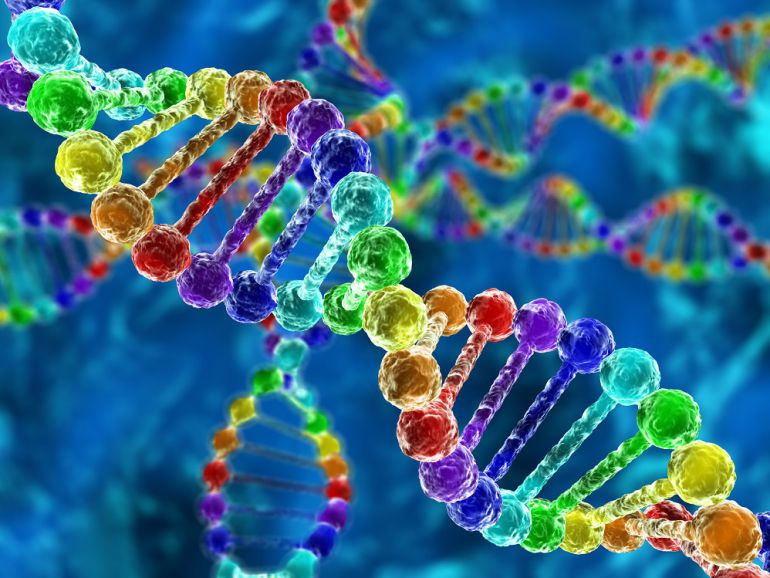
\includegraphics[width=1\linewidth]{Tema1/00_ADN.jpg}
    \caption{ADN}
    \label{fig:adn}
\end{figure}

\section{Qué es un ser vivo}

Llamamos ser vivo a todo aquello que está formado por una o más células y realiza las tres funciones vitales: nutrición, relación y reproducción.

\subsection{Las células y sus tipos}
Una célula  (Figura \ref{fig:celula-eucariota}) es la parte más pequeña de un ser vivo que, a su vez, está viva; es decir, que puede realizar las funciones vitales; se nutre, se relaciona y se reproduce.

\vspace{3mm}
las células de diferentes seres vivos tienen una estructura común con cuatro componentes: la membrana, el citoplasma, el material genético y los orgánulos.

\begin{figure}[ht]
    \centering
    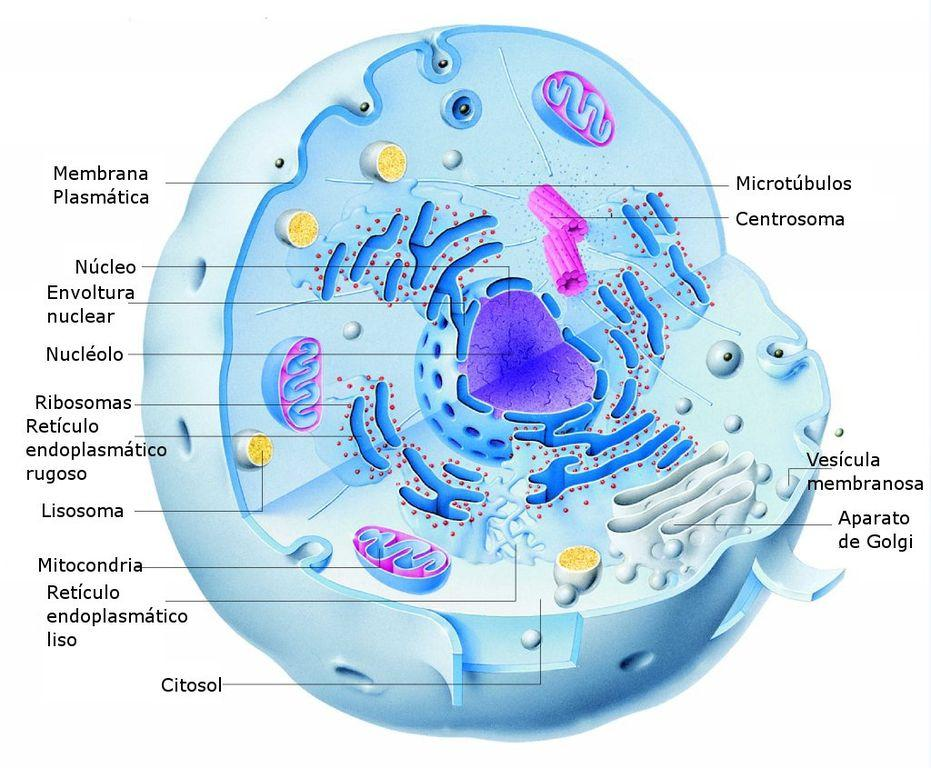
\includegraphics[width=0.7\linewidth]{Tema1/02_Celula_eucariota.jpg}
    \caption{Célula eucariota}
    \label{fig:celula-eucariota}
\end{figure}

\begin{itemize}
    \item \textbf{La membrana plasmática}, que es la envoltura fina y flexible que rodea a la célula y que regula el intercambio de sustancias con el exterior.
    \item \textbf{El citoplasma}, que es el gel que llena el interior de la célula.
    \item \textbf{El material genético}, que es la sustancia fibrosa llamada ADN que dirige el funcionamiento celular.
    \item \textbf{Los orgánulos}, que son estructuras especializadas en determinadas funciones. Según el tipo de células podremos encontrar unos orgánulos u otros.
\end{itemize}

Hay dos tipos principales de células, las \textbf{células procariotas} y las \textbf{células eucariotas}; Las células eucariotas se dividen en dos tipos: las \textbf{eucariotas de tipo animal} y las \textbf{eucariotas de tipo vegetal}.

\vspace{3mm}
Las células procariotas (Figura \ref{fig:celula-procariota}) tienen el material genético libre en el citoplasma, pocos orgánulos y una pared alrededor de la membrana.

\begin{figure}[ht]
    \centering
    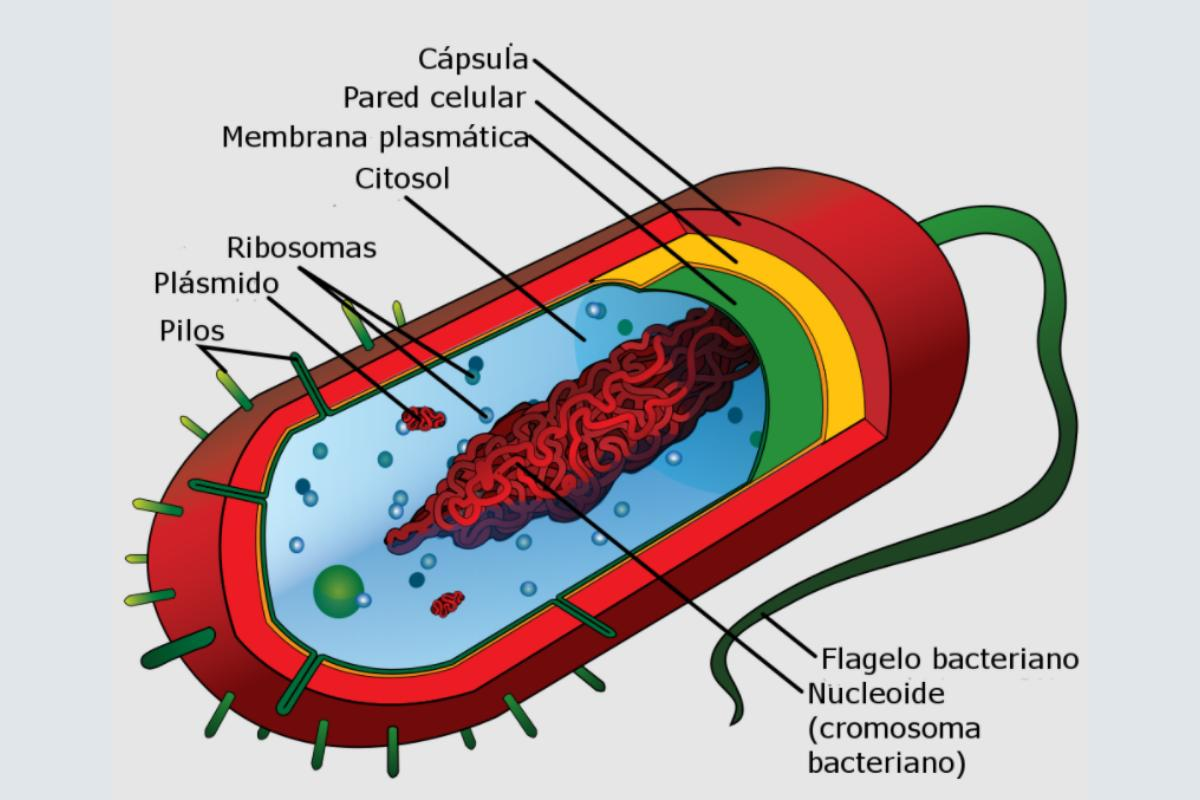
\includegraphics[width=0.6\linewidth]{Tema1/01_Celula_procariota.jpg}
    \caption{Célula procariota}
    \label{fig:celula-procariota}
\end{figure}

Las células eucariotas tienen el material genético rodeado de una membrana, que forma el núcleo, y se componen de una gran variedad de orgánulos.

\vspace{3mm}
Células eucariotas de tipo animal (Figura \ref{fig:eucariota-animal}) son las que tienen todos los animales y algunos organismos
como los protozoos.

\begin{figure}[ht]
    \centering
    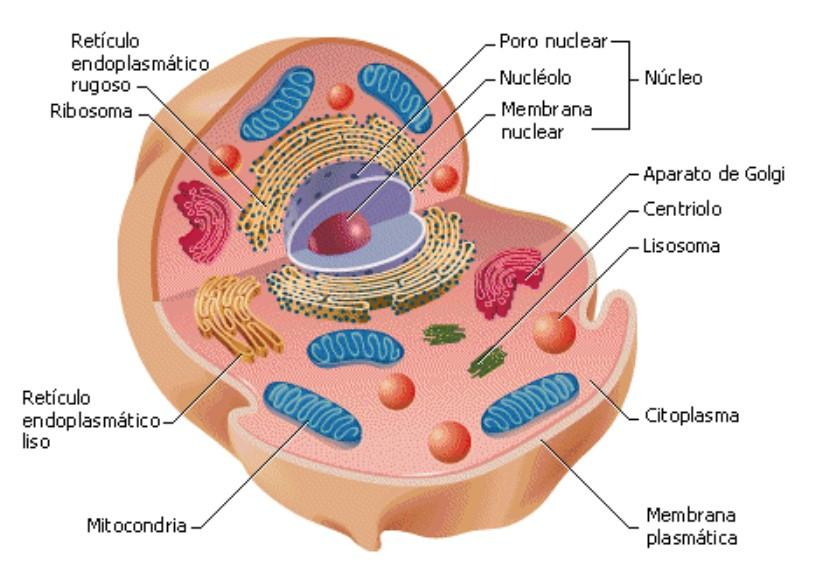
\includegraphics[width=0.6\linewidth]{Tema1/03_Celula_animal.jpg}
    \caption{Célula eucariota animal}
    \label{fig:eucariota-animal}
\end{figure}

\vspace{3mm}
Células eucariotas de tipo vegetal (Figura \ref{fig:eucariota-vegetal}) son las que tienen las plantas y las algas. Tienen una pared rígida y orgánulos especializados en realizar la fotosíntesis, como los cloroplastos.

\begin{figure}[!ht]
    \centering
    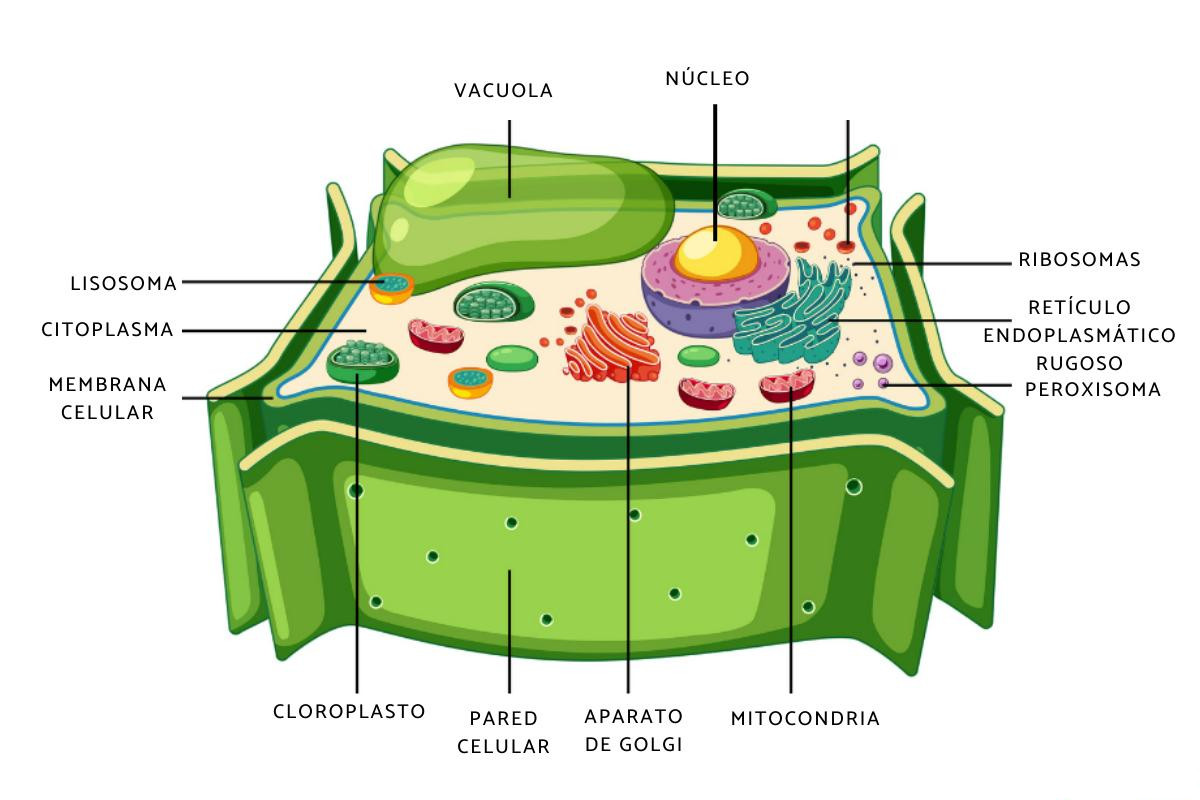
\includegraphics[width=0.7\linewidth]{Tema1/04_Celula_vegetal.jpg}
    \caption{Célula eucariota vegetal}
    \label{fig:eucariota-vegetal}
\end{figure}

\subsection{Las funciones vitales de las células}

Una célula es capaz de realizar las tres funciones vitales: nutrición, relación y reproducción.

\vspace{3mm}
\textbf{Función de nutrición} (Figura \ref{fig:nutricion-celular})

\begin{itemize}
    \item Consiguen nutrientes. Según la forma de obtener los nutrientes, la nutrición puede ser autótrofa o heterótrofa. Las células con nutrición autótrofa los fabrican con agua, dióxido de carbono y energía solar en un proceso llamado fotosíntesis. Las células con nutrición heterótrofa los obtienen de alimentos procedentes de otros seres vivos.
    \item Respiran. La mayoría de las células toman y utilizan el oxígeno del medio.
    \item Utilizan el alimento y el oxígeno. En su interior, las células utilizan los nutrientes y el oxígeno para crecer, para repararse y para obtener energía.
    \item Expulsan los desechos. Tras utilizar los nutrientes y el oxígeno, las células producen
sustancias de desecho que expulsan al exterior
a través de su membrana.
\end{itemize}

\begin{figure}[!ht]
    \centering
    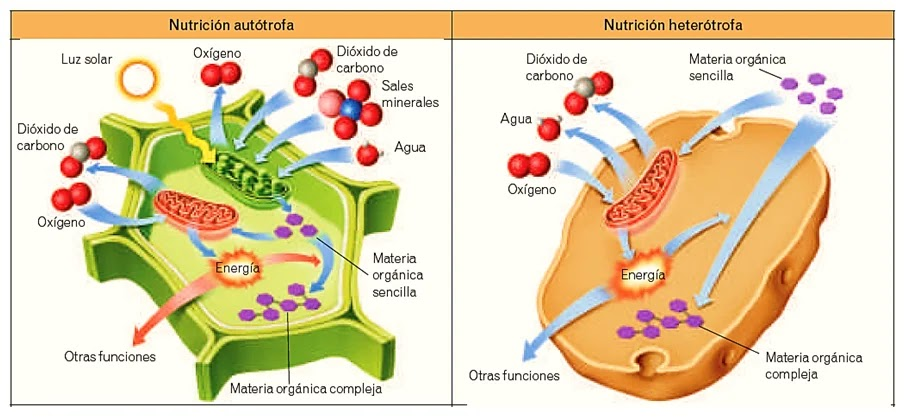
\includegraphics[width=0.8\linewidth]{Tema1/05_Nutricion_celular.jpg}
    \caption{Nutrición celular}
    \label{fig:nutricion-celular}
\end{figure}

\textbf{Función de relación} (Figura \ref{fig:relacion-celular})

Las células son capaces de reaccionar a cambios que se producen dentro o fuera de ella. Algunas son capaces de moverse y desplazarse gracias a ciertas partes especializadas.

\begin{figure}[!ht]
    \centering
    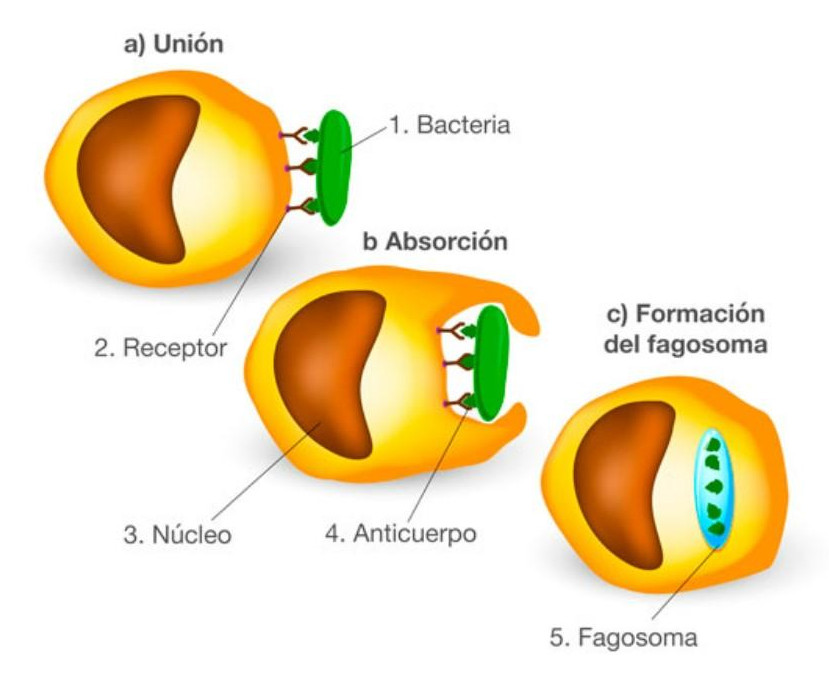
\includegraphics[width=0.5\linewidth]{Tema1/06_Relacion_celular.jpg}
    \caption{Función de relación}
    \label{fig:relacion-celular}
\end{figure}

\textbf{Función de reproducción} (Figura \ref{fig:reproduccion-celular}

Las células pueden formar células hija semejantes a ellas. Para ello, hacen una copia de su material genético y reparten su citoplasma en dos mitades. Material genético y citoplasma se separan y forman dos células.

\begin{figure}[!ht]
    \centering
    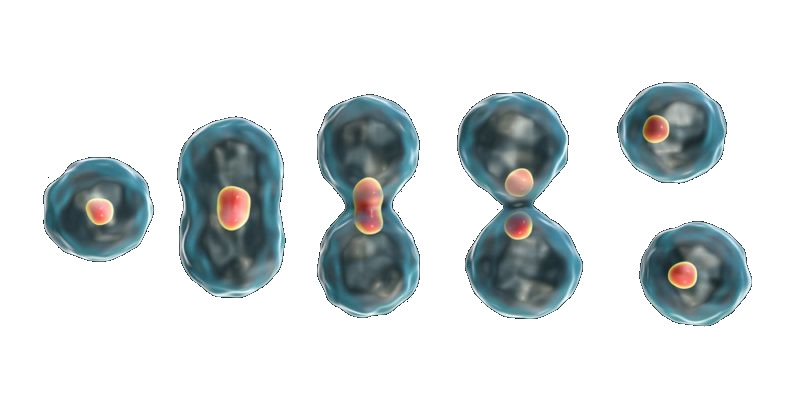
\includegraphics[width=0.6\linewidth]{Tema1/07_Reproduccion_celular.jpg}
    \caption{Función de reproducción}
    \label{fig:reproduccion-celular}
\end{figure}
\section{Niveles de organización}

Los seres vivos pueden tener menor o mayor complejidad, dependiendo del número de células que los componen.

\vspace{3mm}
Los seres vivos \textbf{unicelulares} están formados por una única célula. En estos seres vivos, las tres funciones vitales las lleva a cabo su única célula. Los organismos unicelulares pueden ser procariotas o eucariotas.

\vspace{3mm}
Los seres vivos \textbf{pluricelulares} están formados por varias células más o menos especializadas que funcionan de forma integrada.

\vspace{3mm}
Las células de los seres pluricelulares son eucariotas. En muchos seres vivos, estas células se encuentran asociadas formando tejidos, órganos y aparatos o sistemas (Figura \ref{fig:organizacion-pluricelular}).

\begin{figure}[!ht]
    \centering
    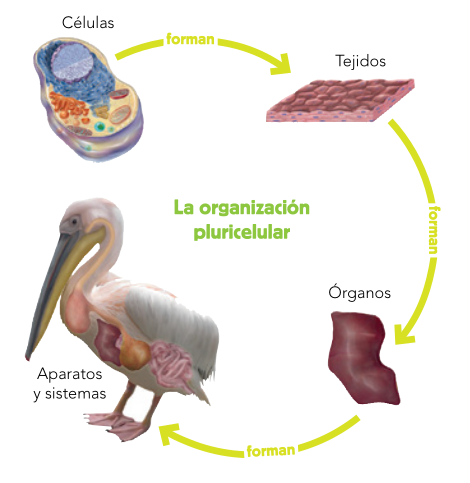
\includegraphics[width=0.5\linewidth]{Tema1/08_Organizacion_pluricelular.png}
    \caption{Organización pluricelular}
    \label{fig:organizacion-pluricelular}
\end{figure}

\begin{itemize}
    \item Los tejidos son agrupaciones de células especializadas en realizar una misma tarea. Por ejemplo, algunos seres vivos tienen tejidos, como el muscular, formado por células especializadas en producir movimientos.
    \item Los órganos son agrupaciones de tejidos que realizan tareas muy especializadas y coordinadas. Por ejemplo, hay seres vivos que tienen órganos como el corazón, que se encarga de bombear la sangre por el cuerpo.
    \item Los aparatos o sistemas son conjuntos de órganos que se agrupan para llevar a cabo un proceso más complejo. Por ejemplo, algunos seres vivos tienen aparatos como el digestivo que realiza el proceso de la digestión, formado por muchos órganos.
\end{itemize}
\section{Los cinco reinos}

Los seres vivos se clasifican en cinco reinos: moneras, protoctistas, hongos, plantas y animales.

\vspace{3mm}
Esta clasificación de los seres vivos en reinos se ha establecido atendiendo a diferentes criterios como: si sus células son procariotas o eucariotas; si son unicelulares o pluricelulares; si tienen o no tejidos, u órganos, y si su nutrición es autótrofa o heterótrofa.

\subsection{Reino de los Moneras}

El reino de los moneras lo forman seres unicelulares procariotas cuya célula carece de núcleo. Pueden realizar una nutrición autótrofa o heterótrofa y a veces forman colonias. Este reino incluye bacterias y otros organismos parecidos a ellas. Las bacterias son los organismos más abundantes de la Tierra. Se encuentran en el aire, en el agua, en el suelo, sobre nuestra piel e, incluso, en el interior de nuestro intestino.

\vspace{3mm}
\textbf{Tipos de bacterias}

Las bacterias (Figura \ref{fig:tipos-bacterias}) tienen un tamaño tan pequeño que solo pueden ser observadas con un microscopio. Sus diferentes formas sirven para clasificarlas:

\begin{itemize}
    \item Algunas tienen forma de esfera; son las llamadas cocos.
    \item Otras tienen forma de bastoncillo; son los bacilos.
    \item Las que tienen forma de coma se llaman vibrios.
    \item Las que adoptan forma de espiral alargada son los espirilos y las espiroquetas.
\end{itemize}

\begin{figure}[!ht]
    \centering
    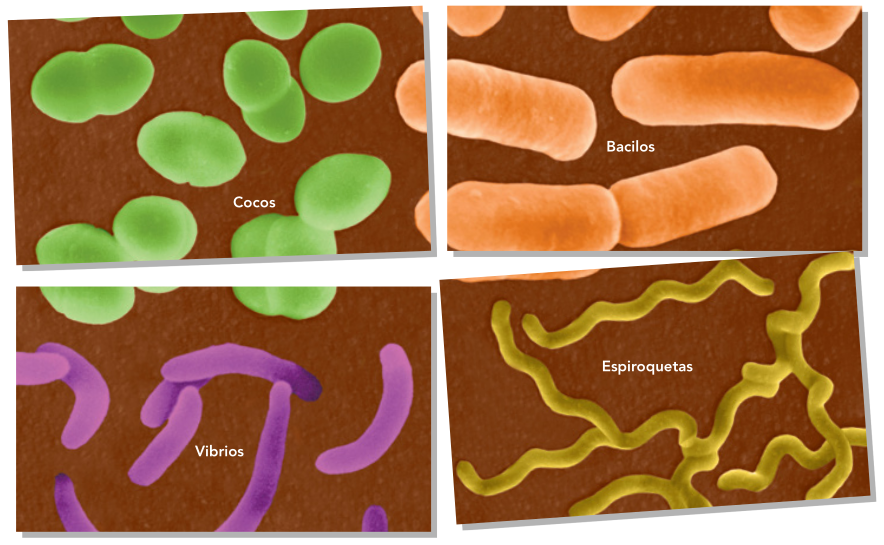
\includegraphics[width=0.7\linewidth]{Tema1/09_Tipos_bacterias.png}
    \caption{Tipos de bacterias}
    \label{fig:tipos-bacterias}
\end{figure}

\textbf{Funciones vitales de las bacterias}

\begin{itemize}
    \item \textbf{Nutrición}

    Las bacterias presentan los dos tipos de nutrición:

    \begin{itemize}
        \item \textbf{Autótrofa.} Hay bacterias que fabrican su alimento a través de la fotosíntesis; por ejemplo, las cianobacterias.
        \item \textbf{Heterótrofa.} Las bacterias con este tipo de nutrición toman el alimento del medio, bien descomponiendo restos de seres vivos, bien a partir de otros seres vivos a los que producen perjuicios o beneficios.
    \end{itemize}
    \item \textbf{Relación}

    Algunas bacterias se desplazan, por ejemplo, mediante flagelos. Otras permanecen inmóviles.
    \item \textbf{Reproducción}

    Las bacterias se reproducen asexualmente por división de su célula. Se multiplican con gran rapidez: en pocas horas pueden pasar de unos centenares a ser millones.
\end{itemize}

\textbf{Las bacterias y el ser humano}

Las bacterias pueden ser perjudiciales para las personas, aunque la mayoría son beneficiosas.

\begin{itemize}
    \item \textbf{Bacterias perjudiciales.} Algunas bacterias invaden nuestro organismo y nos causan enfermedades, como la bronquitis, el cólera o la salmonelosis. Otras contaminan los alimentos y los estropean.
    \item \textbf{Bacterias beneficiosas.} Muchas bacterias se utilizan en las industrias: para fabricar productos alimentarios como el yogur, el queso o el vinagre; o para elaborar medicamentos, como los antibióticos que se usan para curar enfermedades. Otros tipos de bacterias se usan para depurar aguas contaminadas o para eliminar residuos.
\end{itemize}


\subsection{Reino de los Protoctistas}

Son seres con células eucariotas. Los hay unicelulares (protozoos, algas microscópicas...) y pluricelulares que no forman tejidos (grandes algas). Los protozoos realizan nutrición heterótrofa; las algas, autótrofa.

\begin{itemize}
    \item \textbf{Los protozoos} (Figura \ref{fig:tipos-protozoos}). Los protozoos son seres unicelulares y heterótrofos. Viven en medios acuáticos, en tierras húmedas o en el interior de otros seres vivos.

    \textbf{Tipos de protozoos}. Los protozoos pueden clasificarse según las estructuras que utilizan para desplazarse:
    \begin{itemize}
        \item Los hay que emiten unas prolongaciones que salen de su citoplasma llamadas pseudópodos.
        \item Otros tienen un único filamento, llamado flagelo, que mueven a modo de látigo.
        \item Algunos tienen en su superficie pequeños filamentos móviles llamados cilios.
        \item También los hay inmóviles, que carecen de estructuras para desplazarse.
    \end{itemize}

    \begin{figure}[!ht]
        \centering
        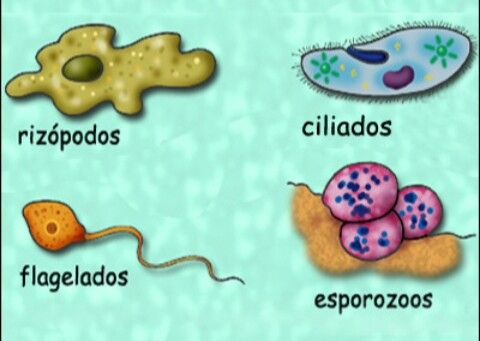
\includegraphics[width=0.65\linewidth]{Tema1/10_Tipos_protozoos.jpg}
        \caption{Tipos de protozoos}
        \label{fig:tipos-protozoos}
    \end{figure}

    \textbf{Funciones vitales de los protozoos}.
    \begin{itemize}
        \item \textbf{Nutrición}. Los protozoos tienen nutrición heterótrofa; algunos se alimentan de residuos que encuentran en el medio; otros son cazadores de microorganismos, de los que se alimentan.
        \item \textbf{Relación}. Muchos son capaces de moverse para capturar el alimento o para acercarse o alejarse de la luz; otros reaccionan expulsando sustancias.
        \item \textbf{Reproducción}. Por lo general, los protozoos se reproducen de forma asexual.
    \end{itemize}

    \textbf{Los protozoos y el ser humano.} Algunos protozoos son perjudiciales, y nos causan enfermedades como la malaria; otros son beneficiosos, como los que forman parte del plancton del que se alimentan muchos seres acuáticos, de los que, a su vez, nos alimentamos las personas.
    
    \item \textbf{Las algas.} Las algas pueden ser unicelulares o pluricelulares y no tienen tejidos. Su nutrición es siempre autótrofa. La gran mayoría de las algas son acuáticas, pero algunas pueden vivir en la corteza de los árboles y sobre las rocas.

    \textbf{Tipos de algas.} Hay algas unicelulares, como las euglenas, que se desplazan en el agua. Las algas pluricelulares, además de clorofila, pueden tener otros pigmentos que les dan un color característico.

    Así, según sea el pigmento mayoritario, se clasificanen (Figura \ref{fig:tipos-algas}):
    \begin{itemize}
        \item Algas verdes, que tienen, sobre todo, clorofila.
        \item Algas rojas, que contienen pigmentos de color rojo.
        \item Algas pardas, con pigmentos anaranjados.
    \end{itemize}

    \begin{figure}[!ht]
        \centering
        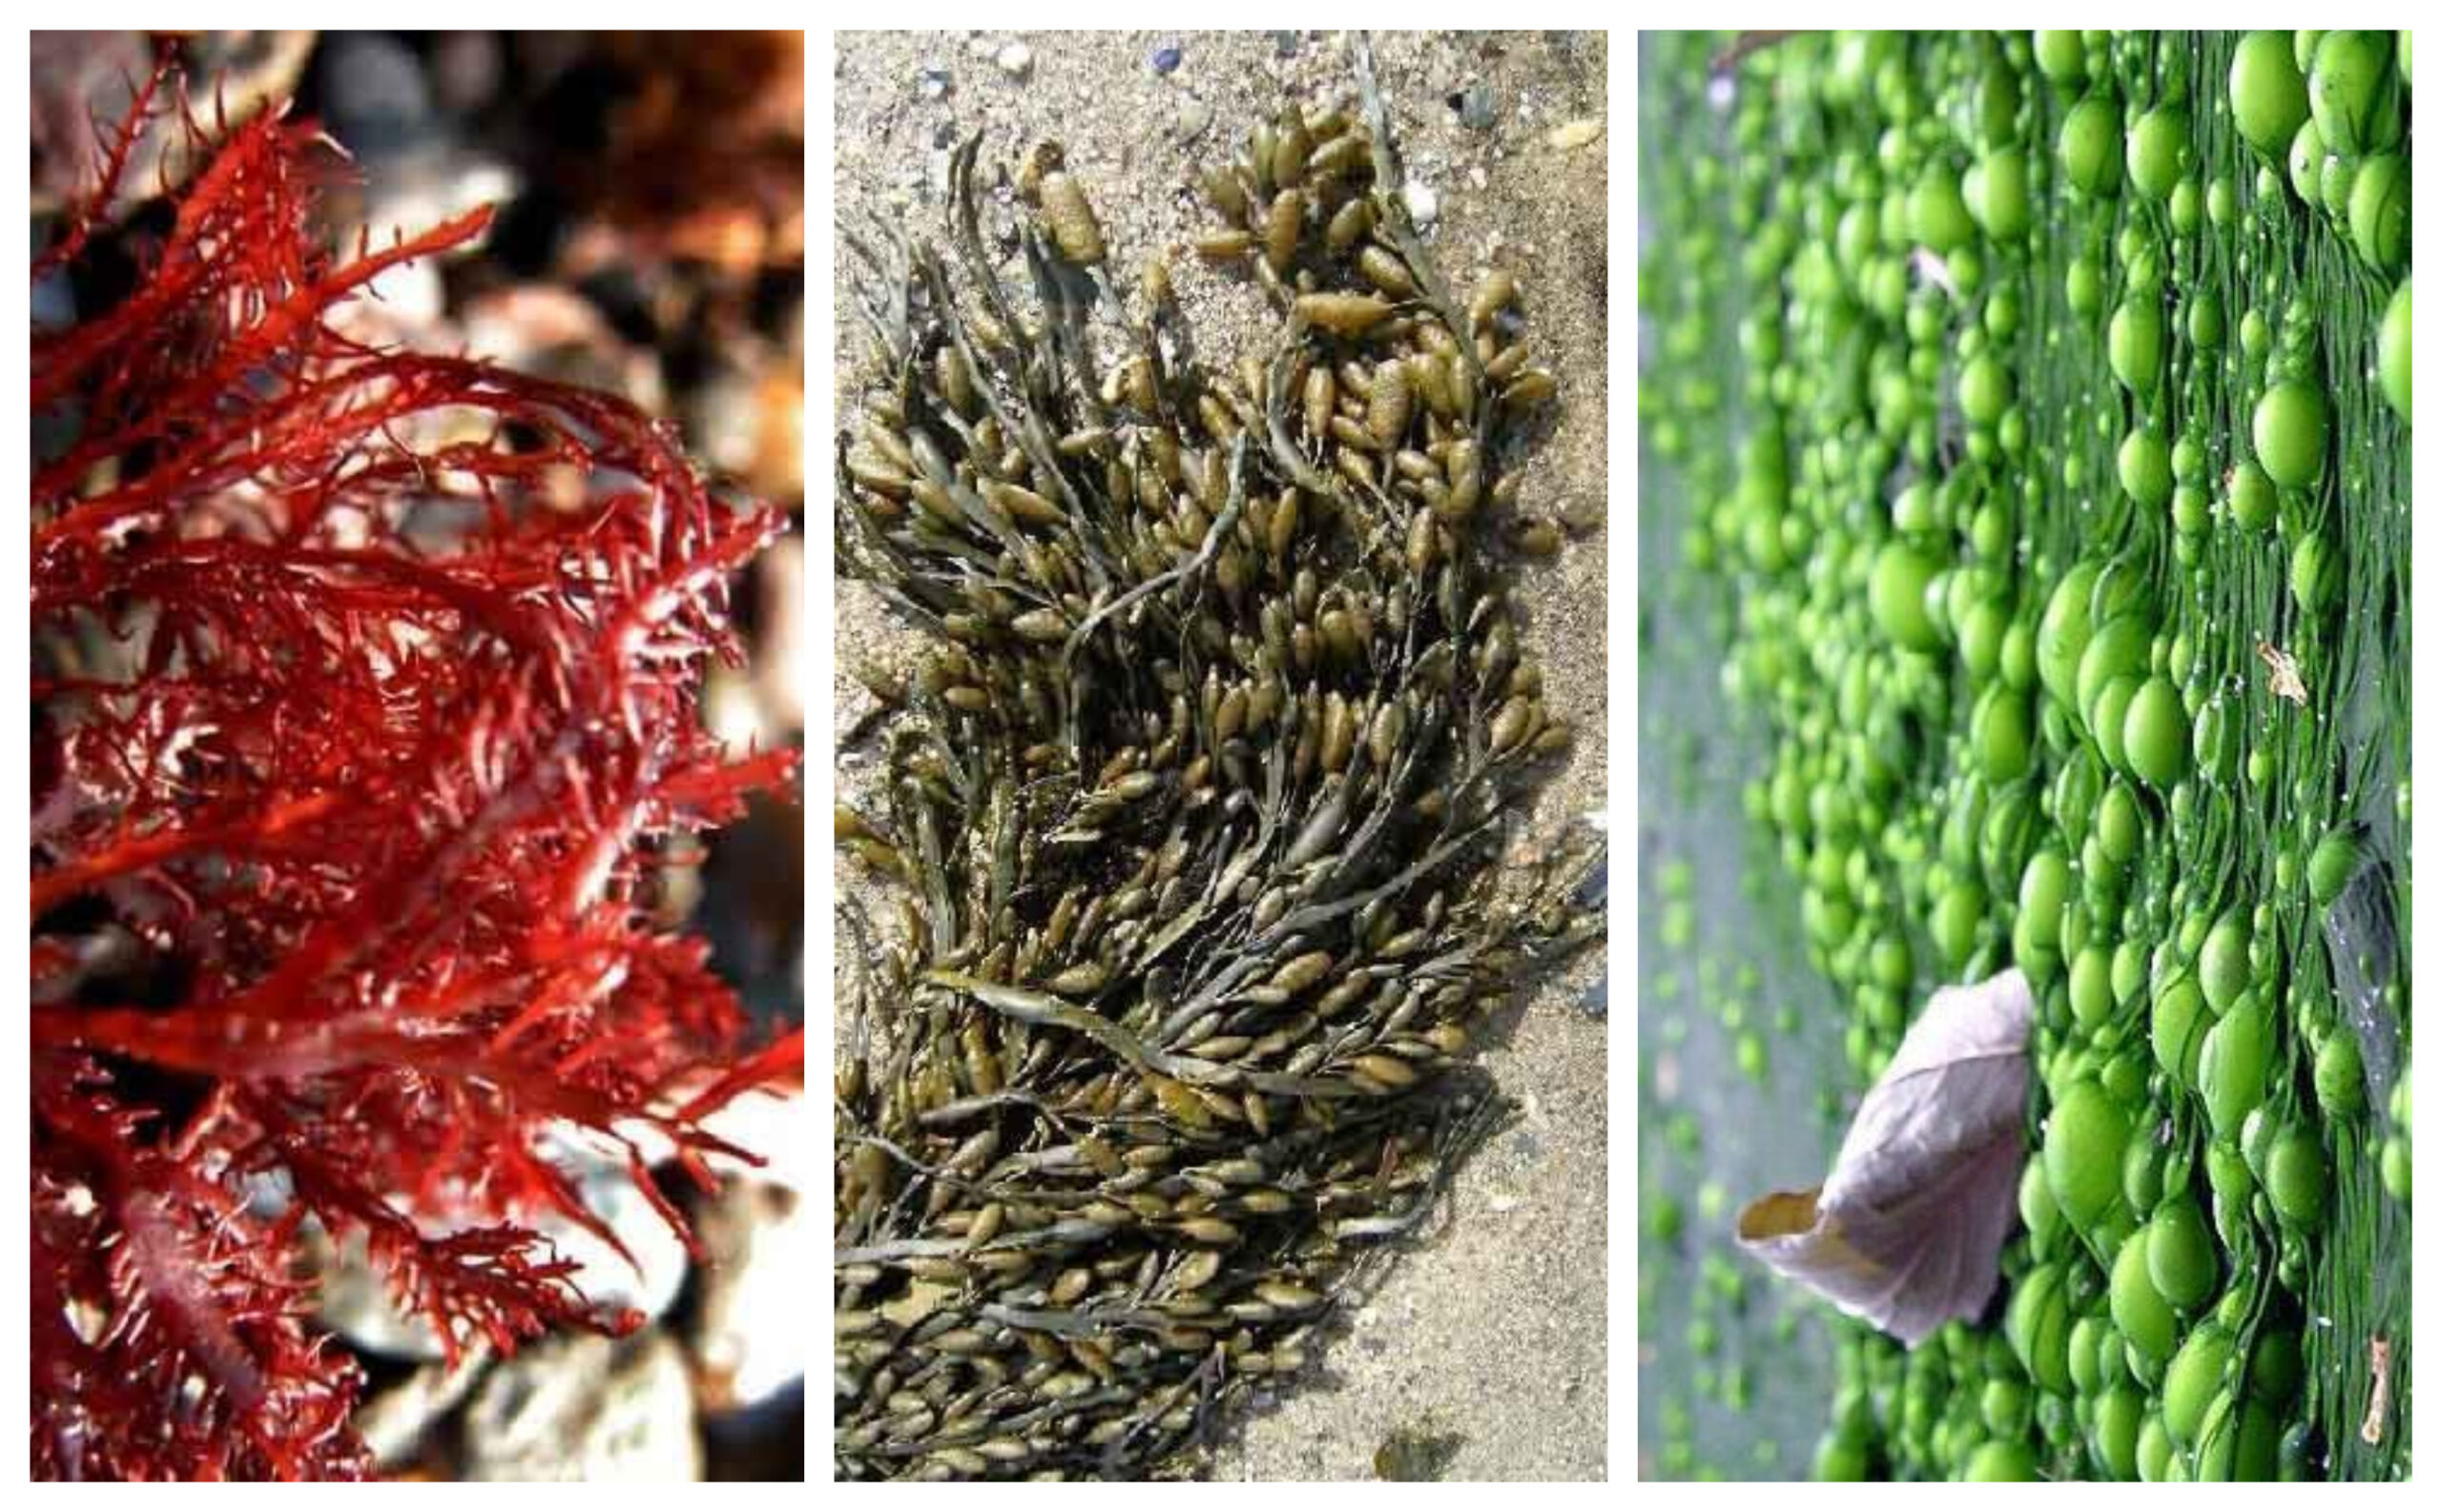
\includegraphics[width=0.65\linewidth]{Tema1/11_Tipos_algas.jpg}
        \caption{Tipos de algas}
        \label{fig:tipos-algas}
    \end{figure}

    \textbf{Funciones vitales de las algas}
    \begin{itemize}
        \item \textbf{Nutrición}. Todas las algas son autótrofas y sintetizan su propia materia orgánica mediante la fotosíntesis.
        \item \textbf{Relación}. Las algas unicelulares tienen flagelos con los que nadan hacia la luz. Las pluricelulares tienen estructuras para fijarse a las rocas y resistir el oleaje o para flotar en la superficie del agua.
        \item \textbf{Reproducción}. Las algas se pueden reproducir de forma asexual y sexual.
    \end{itemize}

    \textbf{Las algas y el ser humano}
    \begin{itemize}
        \item Las \textbf{algas beneficiosas}. Gracias a la fotosíntesis, las algas oxigenan el océano y la atmósfera, reduciendo los niveles de dióxido de carbono. Podemos utilizarlas como alimento o como ingredientes para fabricar batidos o helados. Con otras elaboramos medicamentos, abonos y productos químicos variados.
        \item Las \textbf{algas perjudiciales}. Algunas algas tóxicas, cuando se reproducen en exceso, pueden causar graves problemas de contaminación en mares cerrados, lagos o pantanos.
    \end{itemize}
\end{itemize}

\subsection{Reino de los Hongos}

Los hongos son seres con células eucariotas. Pueden ser unicelulares o pluricelulares que no forman tejidos. Su nutrición es heterótrofa. Los hongos viven en lugares húmedos, con temperaturas suaves y protegidos de la luz.

\vspace{3mm}
\textbf{Tipos de hongos} (Figura \ref{fig:tipos-hongos}). Hay gran variedad de hongos, pero se pueden agrupar en hongos unicelulares, mohos y hongos que forman setas.

\begin{figure}[!ht]
    \centering
    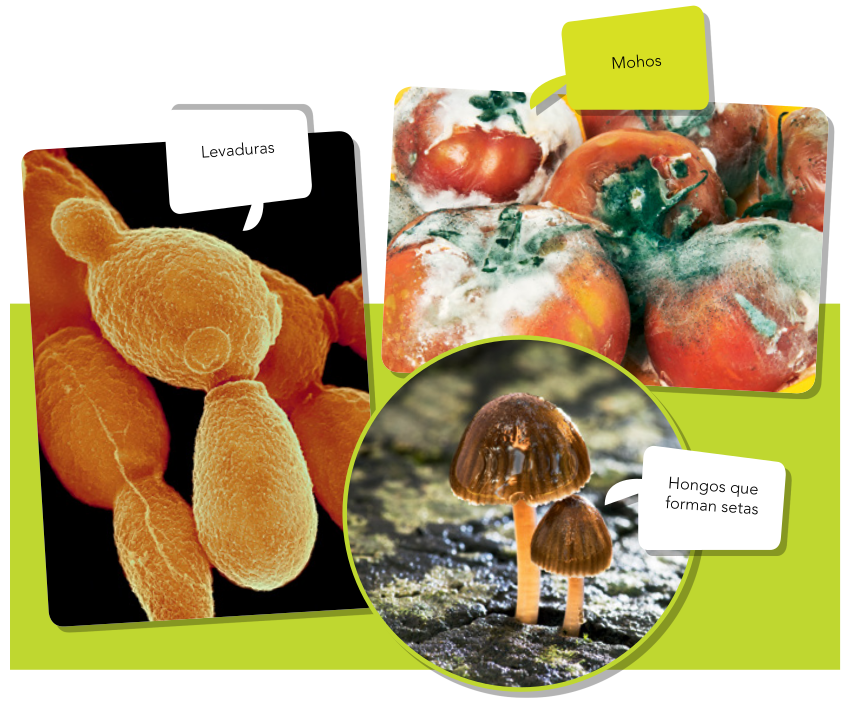
\includegraphics[width=0.6\linewidth]{Tema1/12_Tipos_hongos.png}
    \caption{Tipos de hongos}
    \label{fig:tipos-hongos}
\end{figure}
\begin{itemize}
    \item Los hongos unicelulares, como las levaduras, viven en el suelo, sobre las frutas, en el néctar de las flores...
    \item Los mohos crecen sobre las frutas, el pan o el suelo húmedo. Son pluricelulares y tienen un aspecto parecido al del algodón.
    \item Los hongos que forman setas, como el champiñón o el níscalo, son pluricelulares. Se desarrollan en el suelo, y solo son visibles sus setas.
\end{itemize}

\textbf{Funciones vitales de los hongos}
\begin{itemize}
    \item \textbf{Nutrición.} Los hongos tienen nutrición heterótrofa. Se alimentan de restos de seres vivos. Para ello, se gregan unas sustancias que descomponen el alimento en el exterior del hongo y, posteriormente, absorben los nutrientes.
    \item \textbf{Relación.} Los hongos suelen vivir sobre la superficie o en el interior del suelo, aunque algunos de los unicelulares viven sobre frutas, plantas...
    \item \textbf{Reproducción.} Los hongos unicelulares, como las levaduras, tienen reproducción asexual. Producen descendientes a partir de las yemas o protuberancias que se forman sobre la superficie de su única célula. En la mayoría de los hongos pluricelulares, la estructura reproductora es la seta, que está formada por un pie y un sombrerillo. Este tiene unas laminillas en cuyo interior se generan las denominadas esporas, que al caer al suelo dan origen a nuevos hongos.
\end{itemize}

\textbf{Los hongos y el ser humano}
\begin{itemize}
    \item \textbf{Hongos perjudiciales.} Algunos hongos causan enfermedades a los seres humanos. Otros dañan a las plantas y son capaces de destruir cosechas.
    \item \textbf{Hongos beneficiosos.} De algunos mohos se obtienen antibióticos y otros medicamentos. Algunas setas, como el champiñón o el níscalo, se emplean como alimento; las levaduras se utilizan en la fabricación de alimentos, como el pan, y de bebidas alcohólicas, como el vino. Además, los hongos que viven en el suelo descomponen los restos de seres vivos y forman el humus del que se nutren las plantas.
\end{itemize}

\subsection{Reino de las Plantas}

Las plantas son seres pluricelulares eucariotas cuyas células contienen cloroplastos y tienen una gruesa pared rígida. Tienen tejidos y, casi siempre, órganos. Su nutrición es autótrofa.

\vspace{3mm}
Aunque algunas plantas sencillas, como los musgos, no tienen órganos; la mayoría tiene raíz, tallo, hojas y muchas de ellas, además, flores (Figura \ref{fig:organos-planta}).

\begin{figure}[!ht]
    \centering
    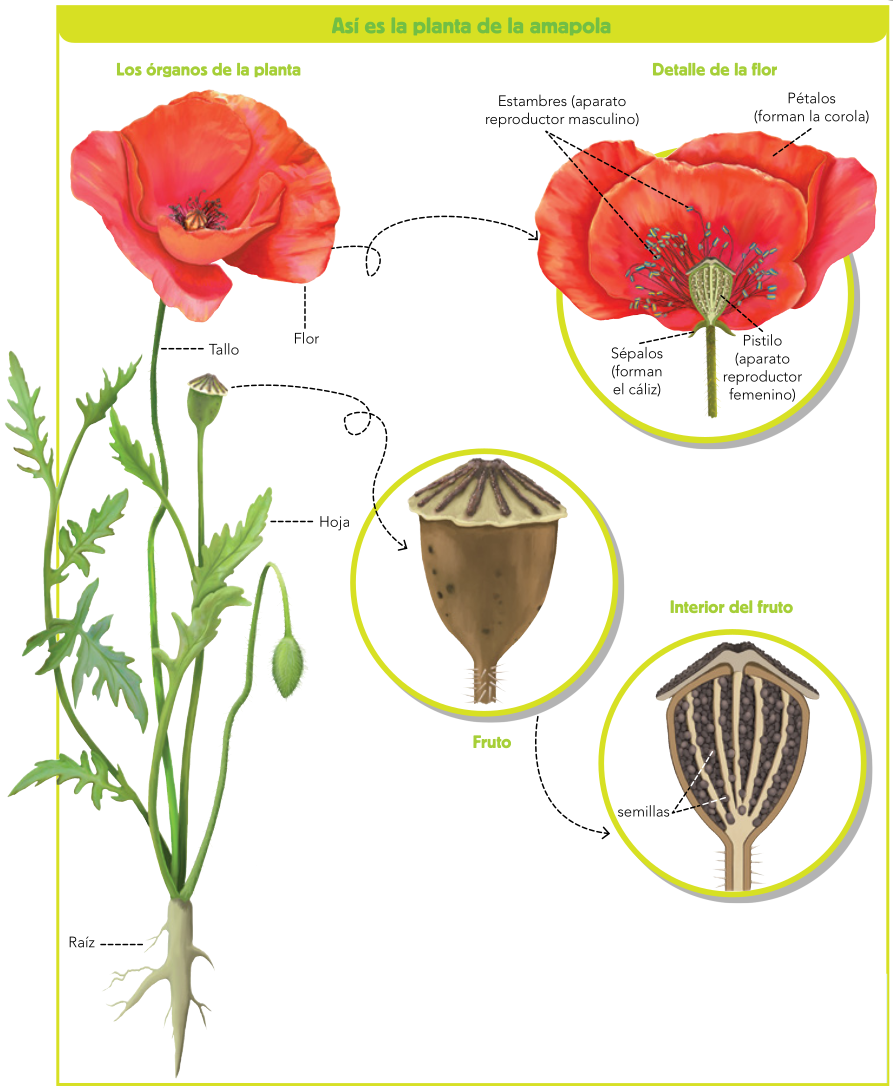
\includegraphics[width=0.8\linewidth]{Tema1/13_Amapola.png}
    \caption{Órganos de una planta y detalle de su flor}
    \label{fig:organos-planta}
\end{figure}

\begin{itemize}
    \item \textbf{La raíz.} Fija la planta al terreno y absorbe agua y minerales...
    \item \textbf{El tallo.} Es el órgano que mantiene erguida a la planta y sostiene las hojas.
    \item \textbf{Las hojas.} Son los órganos especializados en realizar la fotosíntesis.
    \item \textbf{Las flores.} Son los órganos reproductores de algunas plantas. Las más comunes tienen estambres (órganos sexuales masculinos) y pistilo (órgano sexual femenino).
\end{itemize}
La mayoría de las plantas tienen vasos conductores, que son tubos que recorren el interior de la raíz, el tallo y las nerviaciones de las hojas, y por los cuales circulan agua y otras sustancias.

\vspace{3mm}
\textbf{Clasificación}

\vspace{3mm}
Además de la raíz, el tallo, las hojas y las flores, las plantas pueden tener frutos y semillas. Según esto, las plantas se clasifican en plantas sin semillas y plantas con semillas.
\begin{itemize}
    \item \textbf{Plantas sin semillas.} Las plantas sin semillas suelen vivir en lugares muy húmedos. Entre ellas encontramos los musgos, que forman tejidos pero que carecen de raíz, tallo y vasos conductores. Y los helechos, que ya tienen tejidos y órganos.
    \item \textbf{Plantas con semillas.} Las plantas con semillas se clasifican, a su vez, en \textbf{gimnospermas}, cuyas semillas no están encerradas en un fruto, y \textbf{angiospermas}, cuyas semillas están en el interior de un fruto. Algunos ejemplos de gimnospermas son los pinos, los ginkos, las cicas, etc. Algunas angiospermas son el almendro, la retama, el roble, etc.
\end{itemize}

\textbf{Funciones vitales de las plantas} (Figura \ref{fig:funciones-plantas})
\begin{itemize}
    \item \textbf{Nutrición.} Las plantas son autótrofas; es decir, fabrican sus propios nutrientes. Para llevarla a cabo:
    \begin{itemize}
        \item \textbf{Absorben agua y minerales del suelo} que, al mezclarse, forman la savia bruta que sube por el tallo hasta las hojas. Por las hojas entran y salen gases; así, absorben dióxido de carbono del aire.
        \item \textbf{Realizan la fotosíntesis} en las hojas. Para ello, las plantas utilizan la luz solar y fabrican hidratos de carbono (un tipo de nutriente) a partir del agua y del dióxido de carbono. Esos hidratos de carbono se mezclan con la savia bruta formando la savia elaborada, rica en nutrientes, que se distribuye por toda la planta. La fotosíntesis produce oxígeno como desecho.
        \item \textbf{Respiran}, tomando oxígeno y expulsando dióxido de carbono.
        \item \textbf{Eliminan desechos} de su actividad, expulsando de su cuerpo el oxígeno de la fotosíntesis; el dióxido de carbono de la respiración; el exceso de agua, en forma de vapor...
    \end{itemize}
    \item \textbf{Relación.} Las plantas suelen vivir fijas al suelo y, aunque no se desplazan, crecen reaccionando ante la luz o a la gravedad. Detectan los cambios estacionales y algunas pueden moverse si se tocan.
    \item \textbf{Reproducción.} Las plantas tienen órganos reproductores para realizar la reproducción sexual. En la mayoría de ellas los órganos reproductores son las flores. También se pueden reproducir de forma asexual. Algunas lo hacen mediante esporas y, en otros casos, mediante la formación de estructuras especializadas (en las raíces, los tallos o las hojas) que se separan de la planta madre y originan nuevas plantas.
\end{itemize}

\begin{figure}[!ht]
    \centering
    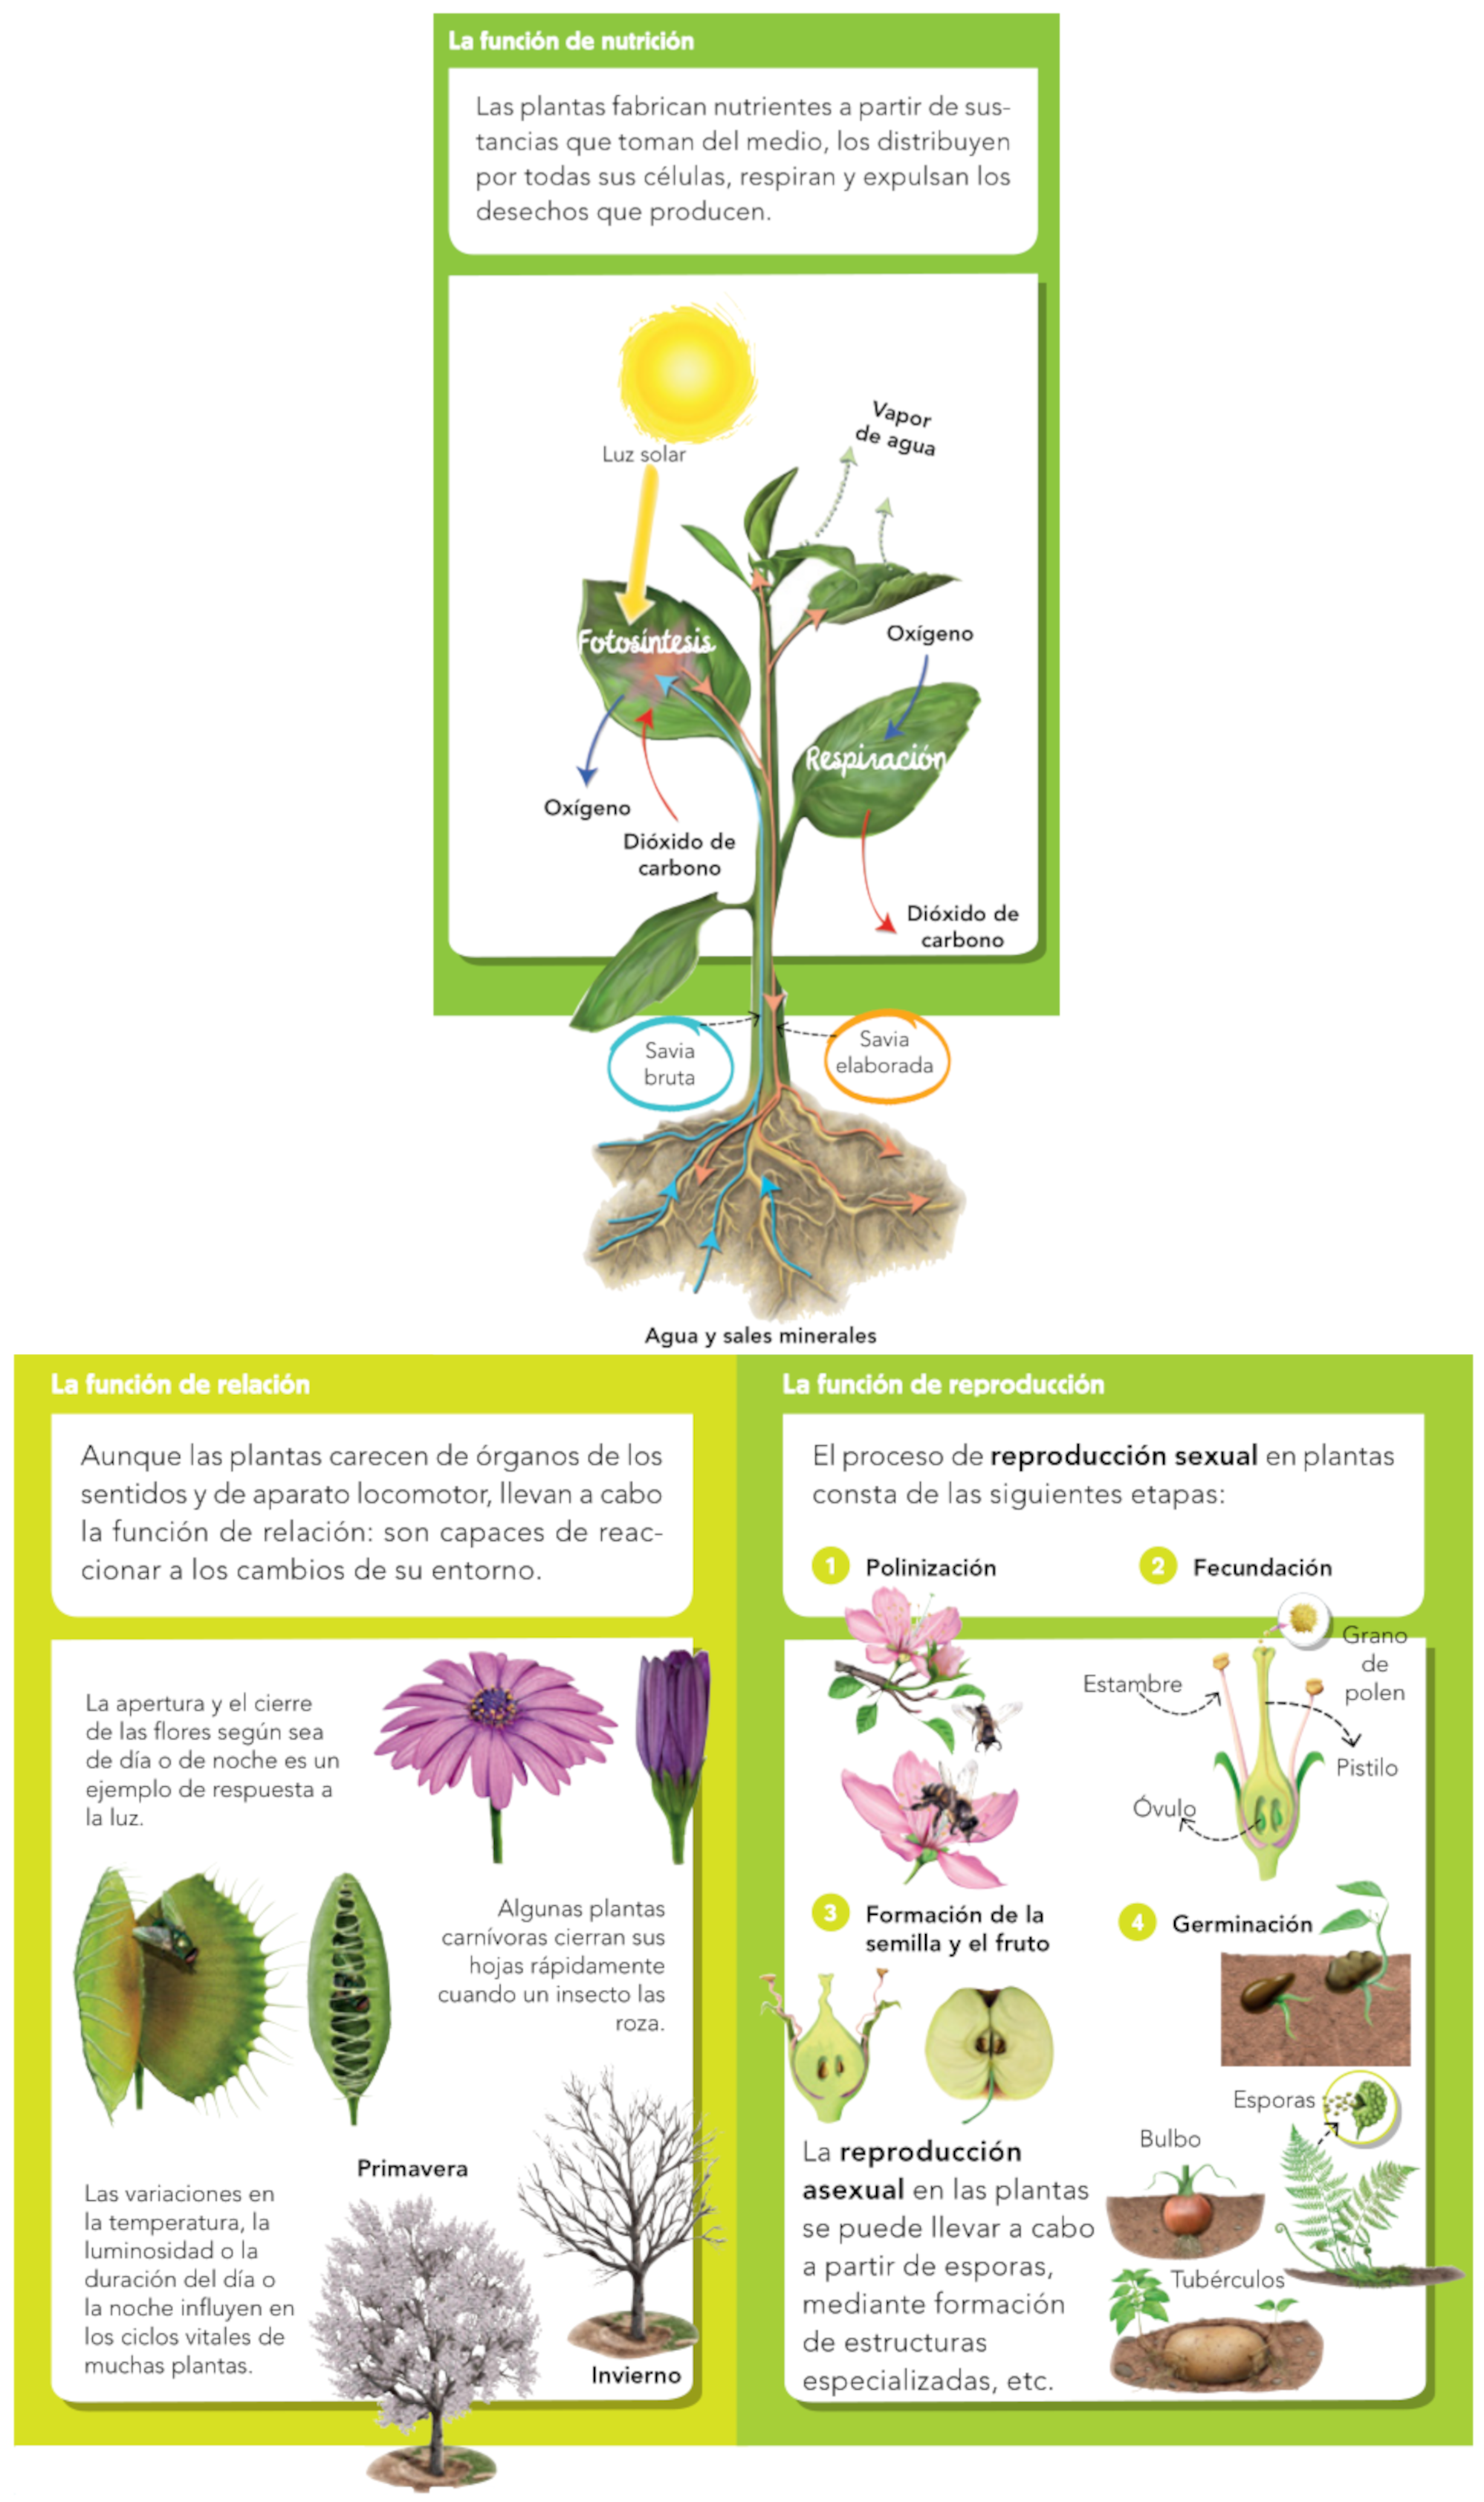
\includegraphics[width=0.7\linewidth]{Tema1/14_Funciones_plantas.png}
    \caption{Funciones vitales de las plantas}
    \label{fig:funciones-plantas}
\end{figure}
\textbf{Las plantas y el ser humano.}

\vspace{3mm}
Las plantas proporcionan numerosos beneficios al medio ambiente, al ser humano y al resto de seres vivos, por lo que debemos respetarlas y conservarlas.
\begin{itemize}
    \item Gracias a la fotosíntesis las plantas producen grandes cantidades de oxígeno $(O_2)$, que necesitamos los seres vivos. En este proceso también consumen dióxido de carbono $(CO_2)$, lo que hace que disminuya el exceso de este gas y, en consecuencia, reducen la contaminación de la atmósfera.
    \item Se emplean como alimento, tanto para el ser humano como para el ganado.
    \item Además, de la madera de las plantas obtenemos celulosa con la que se fabrica papel, corcho, látex, fibras textiles, pigmentos, etc.
    \item Protegen el suelo frente a la erosión gracias a que sus raíces forman una especie de malla. Además, fertilizan el suelo cuando los restos vegetales se descomponen por la acción de los organismos descomponedores.
    \item De ellas se obtienen medicamentos y otras sustancias empleadas en cosmética y perfumería.
    \item Forman entornos muy bellos y llenos de vida, como praderas, bosques, selvas... en los que habitan numerosos seres vivos de todos los reinos.
\end{itemize}
\subsection{Reino de los Animales}

En el reino de los animales se incluyen seres vivos pluricelulares, con células eucariotas de tipo animal, organizadas en tejidos y, casi siempre, órganos, aparatos y sistemas. Su nutrición es heterótrofa.

\subsubsection{Funciones vitales de los animales}
\begin{itemize}
    \item \textbf{Nutrición.} (Figura \ref{fig:nutricion-relacion}).
    \begin{itemize}
        \item \textbf{Alimentación y digestión.} Al ser heterótrofos, los animales deben tomar alimentos procedentes de otros seres vivos. Para ello, cuentan con un aparato digestivo más o menos desarrollado y adaptado para tomar los alimentos y para extraer de ellos los nutrientes.
        \item \textbf{Obtención de oxígeno.} Los animales necesitan tomar oxígeno para utilizarlo en las células. Lo hacen así:
        \begin{itemize}
            \item Los animales acuáticos más sencillos pueden tomar el oxígeno del agua a través de la superficie de su cuerpo; los más complejos lo hacen con unos órganos llamados branquias.
            \item Los animales que toman el oxígeno del aire tienen cavidades en su cuerpo, como las tráqueas (finos tubos ramificados) o los pulmones.
        \end{itemize}
        \item \textbf{Distribución de nutrientes y desechos.} Para transportar los nutrientes a todas sus células y los desechos hasta los órganos que los expulsan, la mayoría de los animales tienen un aparato circulatorio más o menos complicado.
        \item \textbf{Excreción.} Los animales realizan la excreción o expulsión de los desechos del organismo a través de la superficie de su cuerpo o mediante órganos excretores de mayor o menor complejidad.
    \end{itemize}
    \item \textbf{Relación.} (Figura \ref{fig:nutricion-relacion}).
    \begin{itemize}
        \item \textbf{Los órganos de los sentidos.} Los órganos de los sentidos de los animales suelen estar en la cabeza, en caso de tenerla. Con ellos detectan luz (con los ojos), vibraciones sonoras (con los oídos), contacto o calor (con los órganos del tacto), sustancias (con los órganos del olfato y del gusto...), electricidad...
        \item \textbf{Los sistemas nerviosos.} La mayor parte de los animales tiene una red de células nerviosas que conectan todo su cuerpo y lo controlan. Los más complejos tienen nervios y estructuras con mayor capacidad de control, como los ganglios o el cerebro.
        \item \textbf{Los aparatos locomotores.} Los animales tienen tejidos musculares y sistemas de músculos capaces de producir movimientos, además de contar con patas, alas, aletas, que utilizan para desplazarse.
    \end{itemize}
    
    \begin{figure}[!ht]
        \centering
        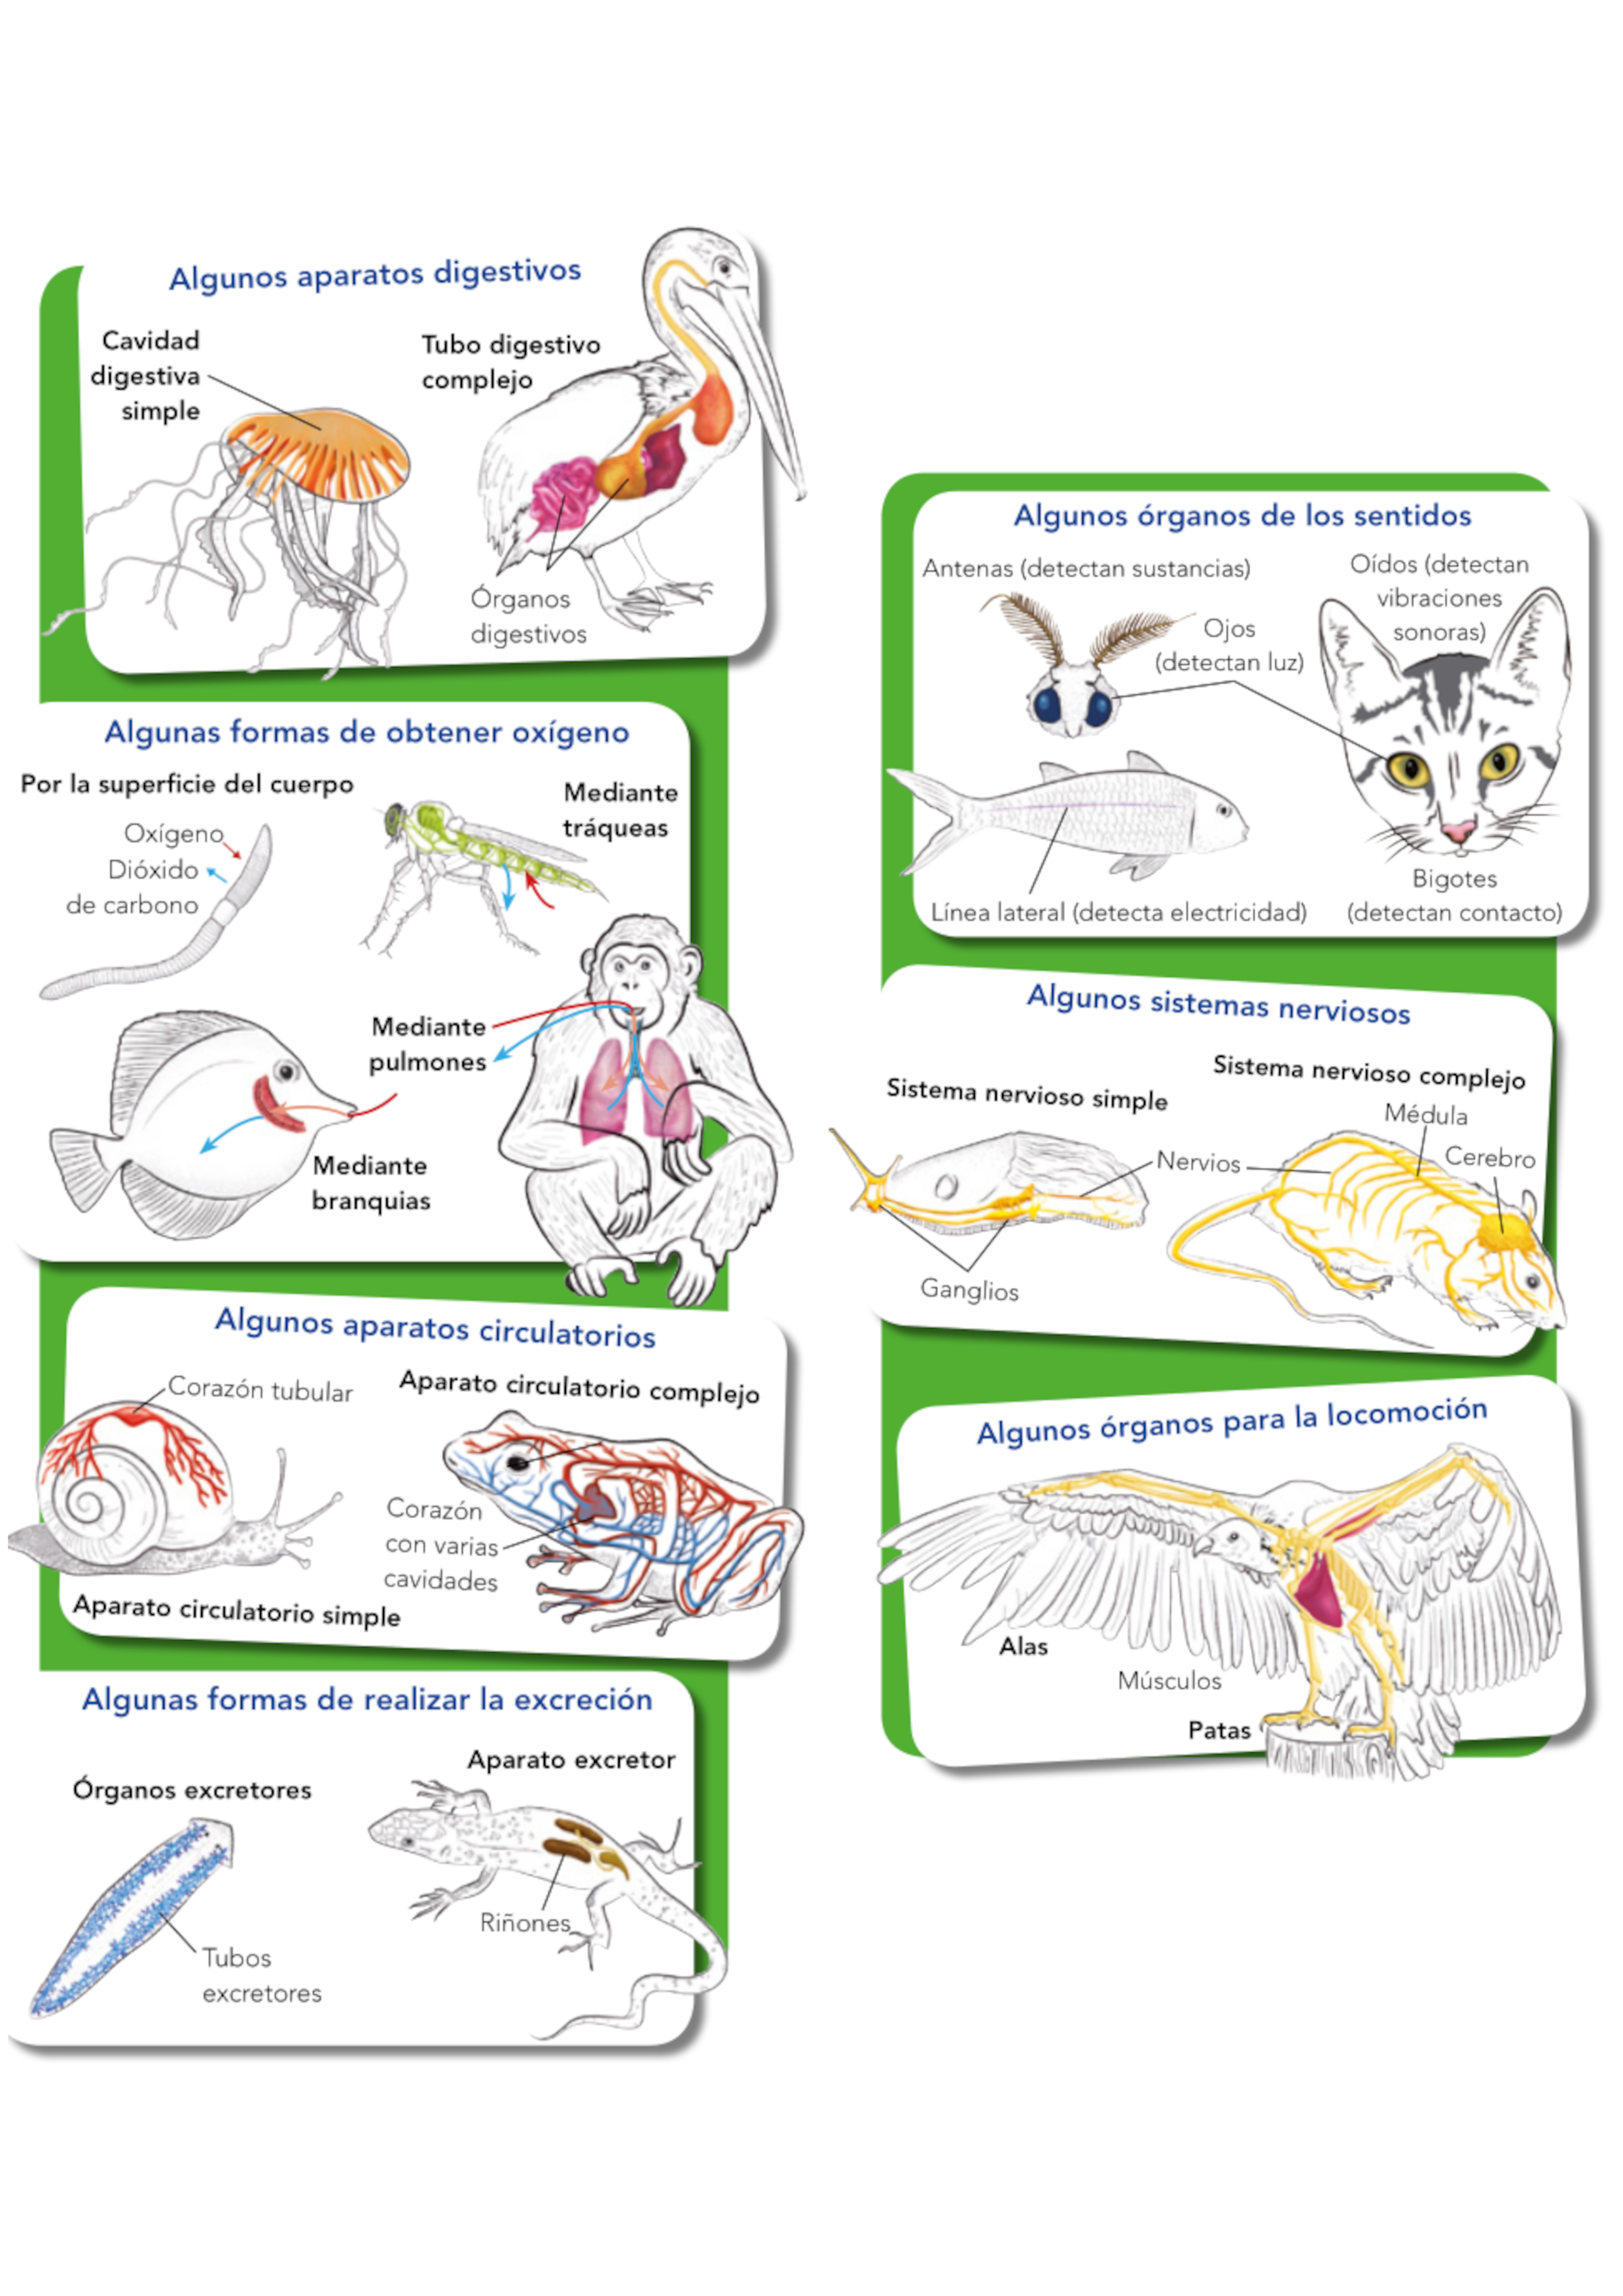
\includegraphics[width=0.7\linewidth]{Tema1/15_Nutricion_relacion.png}
        \caption{Nutrición y relación en los animales}
        \label{fig:nutricion-relacion}
    \end{figure}
    \item \textbf{Reproducción.}

    Los animales realizan una reproducción sexual mediante órganos reproductores que producen células sexuales llamadas gametos. En los animales ovíparos, las crías se desarrollan dentro de huevos, de los que eclosionan. En los vivíparos, las crías maduran en el cuerpo de la hembra, de la que nacen mediante el parto. Ademas, algunos animales simples tienen reproducción asexual y producen descendientes a partir de partes de su cuerpo.
\end{itemize}

\subsubsection{Organización del cuerpo de los animales}

El reino de los animales incluye una gran variedad de seres con mayor o menor grado de organización. Los hay muy simples, como una esponja o una medusa, o muy complejos, como un insecto o un gato, pero casi todos presentan simetría, que puede ser radial o bilateral (Figura \ref{fig:simetria-animal}).

\begin{figure}[!ht]
    \centering
    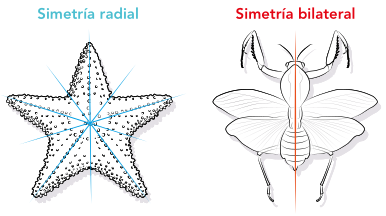
\includegraphics[width=0.5\linewidth]{Tema1/16_Simetria_animal.png}
    \caption{La simetría en los animales}
    \label{fig:simetria-animal}
\end{figure}

\subsubsection{Clasificación de los animales}

La zoología divide el reino de los animales en numerosos grupos. En función de su estructura corporal, hay dos grandes tipos de animales: los invertebrados y los vertebrados (Figura \ref{fig:caracteristicas-animales}).

\begin{figure}[!ht]
    \centering
    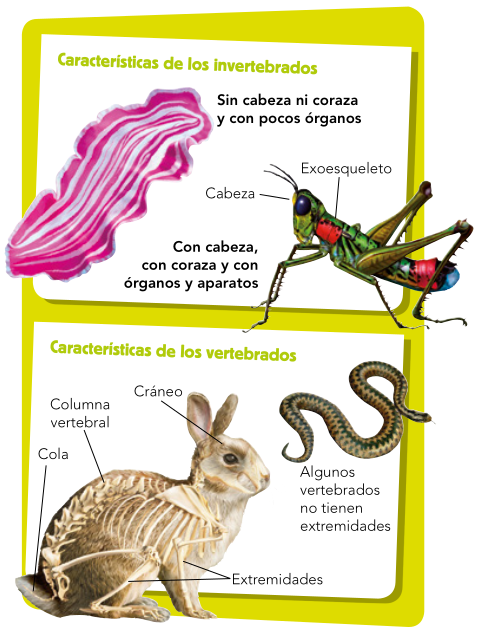
\includegraphics[width=0.4\linewidth]{Tema1/17_Caracteristicas_animales.png}
    \caption{Características de los animales}
    \label{fig:caracteristicas-animales}
\end{figure}

\vspace{3mm}
\textbf{Los invertebrados} (Figura: \ref{fig:invertebrados})

\vspace{3mm}
La mayor parte de los animales son invertebrados. Hay muchos tipos; los más conocidos son los poríferos, los cnidarios, los anélidos, los equinodermos, los moluscos y los artrópodos. Todos ellos carecen de un esqueleto interno con columna vertebral, pero su organización corporal puede ser diversa:
\begin{itemize}
    \item Los más simples, como las medusas, no tienen cabeza diferenciada y muy pocos órganos.
    \item Los más complejos, como los insectos, suelen tener una cabeza definida, con boca, y órganos y aparatos variados bien diferenciados.
\end{itemize}

\begin{figure}[!ht]
    \centering
    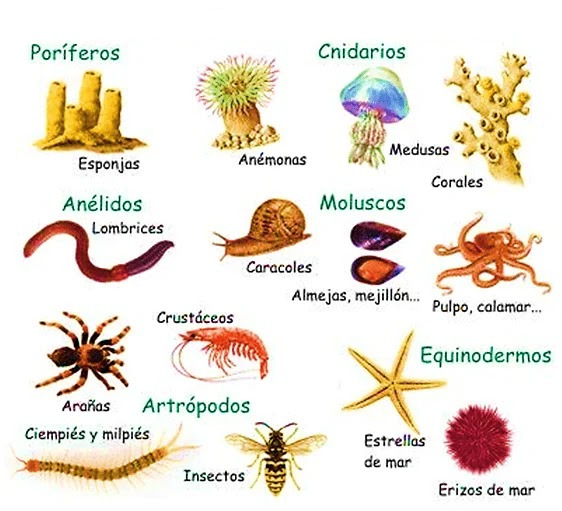
\includegraphics[width=0.7\linewidth]{Tema1/18_Invertebrados.jpg}
    \caption{Invertebrados}
    \label{fig:invertebrados}
\end{figure}

Muchos tienen conchas, corazas, caparazones o exoesqueletos que protegen su cuerpo. Hay numerosos grupos:
\begin{itemize}
    \item \textbf{Los poríferos}. Los poríferos o esponjas son acuáticos y muy sencillos. Su cuerpo, gelatinoso o fibroso, está perforado por numerosos poros y atravesado por canales. Viven fijos en los fondos.
    \item \textbf{Los cnidarios}. Los cnidarios, como las medusas, las anémonas o los corales, son acuáticos. Su cuerpo tiene forma de saco, con una única abertura o boca. Se alimentan de otros animales, que atrapan gracias a unos tentáculos venenosos que rodean la boca. Toman el oxígeno del agua por toda la superficie del cuerpo.
    \item \textbf{Los anélidos}. Hay anélidos acuáticos, como las sanguijuelas, o terrestres como las lombrices. Tienen un cuerpo largo, delgado y musculoso, dividido en anillos. Casi todos tienen una cabeza definida, con una boca que puede tener piezas duras. Toman oxígeno por toda la superficie de su cuerpo.
    \item \textbf{Los equinodermos}. Los equinodermos, como las estrellas o los erizos de mar, son marinos. Su cuerpo, sin cabeza, está cubierto por unas placas espinosas. En su interior, hay un sistema de tubos llenos de líquido, que acaban en pequeños tentáculos que salen al exterior, con los que se desplazan, se alimentan o respiran.
    \item \textbf{Los moluscos}. Entre los moluscos se incluyen animales terrestres o acuáticos. Son los caracoles, las babosas, los mejillones, los pulpos, los calamares... Estos seres tienen el cuerpo dividido en tres partes: cabeza, masa visceral y pie.
    \begin{itemize}
        \item \textbf{La cabeza.} Está más o menos definida según las especies y cuenta con una boca que puede tener dientes o picos para trocear el alimento y órganos de los sentidos para percibir olores, sabores, luz, contacto, etc.
        \item \textbf{La masa visceral.} Contiene los órganos internos y está cubierta por una pared carnosa llamada manto.
        \item \textbf{El pie.} Es un órgano locomotor muy musculoso que puede tener formas muy diversas (aplanada, de hacha, de corona de tentáculos) según los diferentes tipos de moluscos.
    \end{itemize}
    El cuerpo de muchos moluscos está recubierto por una concha, aunque otros carecen de ella. Los moluscos acuáticos toman oxígeno del agua mediante branquias. Los terrestres lo obtienen del aire a través de una cavidad respiratoria que funciona como un pulmón muy simple.
    \item \textbf{Los artrópodos}. El cuerpo de los artrópodos está cubierto por un exoesqueleto articulado; es decir, una coraza de piezas rígidas unidas por juntas flexibles. También tienen una cabeza diferenciada y un tronco segmentado con varios pares de patas.
    \begin{itemize}
        \item \textbf{La cabeza.} En ella están los órganos de los sentidos. Destacan las antenas o los palpos, que son los órganos del olfato y del tacto. Los órganos de la visión constan de dos o más ojos simples (formados por una sola lente sencilla) o de dos ojos compuestos (formados por numerosas lentes que funcionan juntas).
        \item \textbf{El tronco.} Está dividido en más o menos partes o segmentos según el tipo de artrópodo. Contiene los órganos internos y de él salen las patas y, en algunos insectos, las alas.
        \item \textbf{Las patas.} Salen de los segmentos del tronco y pueden tener diversas formas dependiendo de si sirven para el desplazamiento, para agarrarse, para la locomoción... Su número varía en los diferentes grupos de artrópodos.
    \end{itemize}
    Muchos artrópodos acuáticos tienen branquias. Los demás toman oxígeno del aire mediante finos tubos, las tráqueas, abiertos al exterior y comunicados con sus órganos internos.
\end{itemize}

\vspace{3mm}
\textbf{Los vertebrados} (Figura \ref{fig:vertebrados})

\vspace{3mm}
Los animales de este grupo son menos numerosos pero más complejos que los invertebrados. Son los peces, los anfibios, los reptiles, las aves y los mamíferos. Tienen esqueleto interno con:
\begin{itemize}
    \item Una columna vertebral que recorre el tronco y se prolonga, casi siempre, en una cola.
    \item Un cráneo rígido en la cabeza, que protege el cerebro. En la cabeza se hallan la boca y muchos de los órganos de los sentidos.
    \item Cuatro extremidades de diversa morfología, aunque en algunas especies faltan.
\end{itemize}
\begin{figure}[!ht]
    \centering
    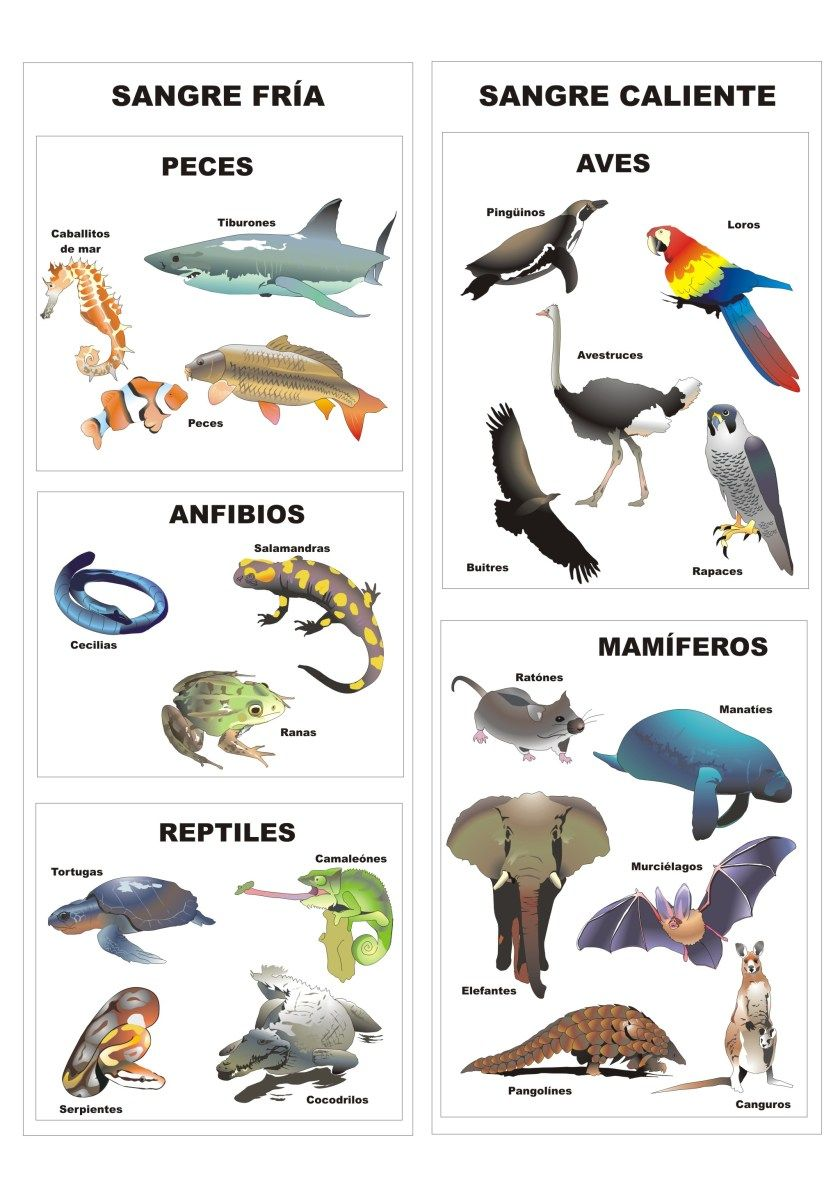
\includegraphics[width=0.7\linewidth]{Tema1/19_Vertebrados.jpeg}
    \caption{Vertebrados}
    \label{fig:vertebrados}
\end{figure}
Hay cinco grupos de vertebrados: peces, anfibios, reptiles, aves y mamíferos.
\begin{itemize}
    \item \textbf{Los peces.} Los peces son animales acuáticos. Su cuerpo está cubierto de escamas y tiene forma hidrodinámica, lo que favorece su avance en el agua. En el tronco y en las extremidades tienen aletas para impulsarse y maniobrar. Los peces toman el oxígeno disuelto en el agua gracias a las branquias. Casi todos los peces son ovíparos y ponen los huevos en el agua. Estos no tienen cáscara, de modo que se secarían en tierra.
    \item \textbf{Los anfibios.} Los anfibios son animales terrestres, pero deben vivir cerca de medios acuáticos o húmedos, ya que su piel fina y desnuda tiende a desecarse. Suelen tener cuatro patas y dedos sin uñas. Son carnívoros. Respiran el oxígeno del agua a través de la piel. Muchos tienen, además, branquias, al menos al nacer, y otros tienen pulmones que les permiten respirar fuera del agua. Casi todos los anfibios son ovíparos; ponen huevos sin cáscara en el agua o en lugares muy húmedos; de no ser así, se desecarían. Las crías respiran en el agua y tienen aletas. Generalmente, se transforman en adultos mediante un conjunto de cambios, llamado metamorfosis, en el que desarrollan patas y la capacidad para salir del agua y respirar oxígeno del aire.
    \item \textbf{Los reptiles.} La mayor parte de los reptiles son terrestres. Pueden sobrevivir en lugares muy secos y alejados del agua gracias a su gruesa piel cubierta por escamas impermeables, diferentes de las de los peces. Su cuerpo termina en una cola y, salvo en el caso de las serpientes, tiene cuatro extremidades acabadas en cinco dedos con uñas. Las extremidades de los reptiles se insertan a los lados del cuerpo, lo que les obliga a desplazarse arrastrándose; este movimiento recibe el nombre de reptación. Respiran mediante pulmones. Casi todos los reptiles son ovíparos y pueden poner sus huevos lejos del agua, ya que estos tienen una cáscara impermeable que evita que se desequen.
    \item \textbf{Las aves.} Las aves son generalmente terrestres. Su cuerpo está cubierto de plumas. Otras de sus características son:
    \begin{itemize}
        \item Una cabeza pequeña, con ojos muy grandes y de gran agudeza visual. En la boca tienen un pico cuya forma varía según la alimentación.
        \item Un cuello largo y flexible, que permite gran movilidad a la cabeza.
        \item Huesos huecos, con refuerzos internos, que consiguen un esqueleto ligero aunque resistente.
        \item Las extremidades delanteras son alas y, salvo en algunos casos como el de los pingüinos o las avestruces, están provistas de plumas de vuelo. Sus patas traseras tienen cuatro dedos con uñas y están recubiertas de escamas.
        \item Las aves toman el oxígeno del aire a través de los pulmones.
        \item Son ovíparas y ponen huevos con cáscara rígida, que incuban para mantenerlos calientes.
        \item Aunque la mayoría de las aves son grandes voladoras, algunas no pueden volar. Por ejemplo, la gallina, el avestruz o el emú no vuelan pero son grandes corredoras.
    \end{itemize}
    \item \textbf{Los mamíferos.} La característica principal de los mamíferos es que las hembras alimentan a sus crías recién nacidas con la leche que producen sus mamas. Son animales terrestres o acuáticos. Suelen tener el cuerpo total o parcialmente cubierto de pelo, que les ayuda a mantener constante su temperatura. En la cabeza tienen órganos de los sentidos y una boca con dientes de diversos tipos. Cada especie tiene una combinación de dientes diferente según se trate de herbívoros, de carnívoros o de omnívoros. Tienen cuatro extremidades, cuya forma varía según su tipo de locomoción: andar, correr, nadar, saltar, trepar, volar, etc. Los mamíferos toman el oxígeno del aire a través de los pulmones. Casi todos los mamíferos son vivíparos; es decir, sus crías se desarrollan en el aparato reproductor de las hembras y nacen mediante un parto. Hay unas pocas especies ovíparas que ponen huevos con cáscara semejantes a los de los reptiles; son, por ejemplo, el ornitorrinco y los equidnas.
\end{itemize}
\section{Ecosistemas}

Todos los seres vivos se distribuyen en los medios formando parte de ecosistemas. (Figura \ref{fig:tipos-ecosistemas})

\begin{figure}[!ht]
    \centering
    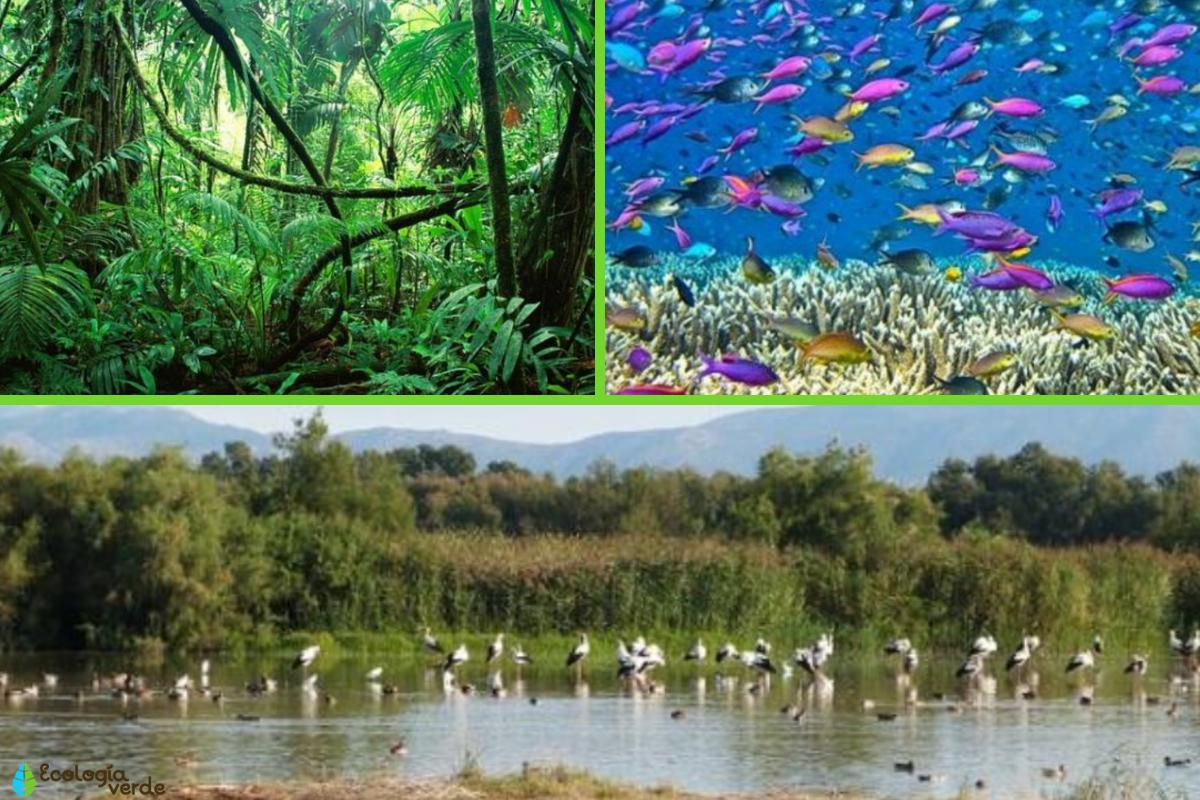
\includegraphics[width=0.7\linewidth]{Tema1/20_Tipos_ecosistemas.jpg}
    \caption{Tipos de ecosistemas}
    \label{fig:tipos-ecosistemas}
\end{figure}

\subsection{Elementos de los ecosistemas}

Un \textbf{ecosistema} es un conjunto formado por un lugar y sus condiciones físicas (llamado \textbf{biotopo}), por una comunidad de seres vivos de varios tipos (llamada \textbf{biocenosis}) y por las relaciones que se dan entre todos estos elementos.

\begin{itemize}
    \item El \textbf{biotopo}. El \textbf{biotopo} de un ecosistema es el conjunto formado por los componentes no vivos de un lugar, como las rocas y el suelo, el aire y el clima, el agua, la luz... Estos componentes varían mucho de unos lugares a otros y determinan que existan varios tipos de ecosistemas, con comunidades de seres vivos propias de esas condiciones.
    \item La \textbf{biocenosis}. La \textbf{biocenosis} o comunidad es el conjunto completo de seres vivos que forman parte de un ecosistema. A su vez, la comunidad de seres vivos de un ecosistema está formada por varias poblaciones. Una \textbf{población} es un conjunto de seres vivos de una misma especie que vive en un ecosistema.
\end{itemize}

\subsection{Relaciones y equilibrio}

En todo ecosistema se dan relaciones entre sus elementos (Figura \ref{fig:relaciones-alimentarias-ecosistema}). Por ejemplo, entre todos los seres vivos y el agua, entre el suelo y las plantas, entre unos seres vivos y otros... Si las relaciones en un ecosistema se mantienen estables y permiten la supervivencia de los seres vivos que lo componen, se dice que ese ecosistema está en \textbf{equilibrio}. De entre todas las relaciones que se dan en un ecosistema, se pueden destacar las \textbf{relaciones alimentarias} o \textbf{tróficas}, que se dan cuando los seres vivos intentan obtener los nutrientes que necesitan. Según esto, los seres vivos de un ecosistema pueden ser:
\begin{itemize}
    \item \textbf{Productores}. Son los seres vivos con \textbf{nutrición autótrofa}, como las \textbf{plantas}, las \textbf{algas} o algunas \textbf{bacterias}. Estos seres son capaces de fabricar (producir) sus nutrientes a partir de agua, dióxido de carbono y minerales que toman del biotopo.
    \item \textbf{Consumidores}. Son los seres vivos con \textbf{nutrición heterótrofa}, como los \textbf{animales} y algunos \textbf{protozoos}, que deben alimentarse de otros seres vivos o de sus partes para obtener nutrientes.
    \item \textbf{Descomponedores}. Son \textbf{bacterias} y \textbf{hongos} capaces de obtener nutrientes y energía \textbf{descomponiendo los restos de seres vivos} en sustancias como agua, gases y minerales, que devuelven al medio para que las utilicen los demás seres vivos.
\end{itemize}

\begin{figure}[!ht]
    \centering
    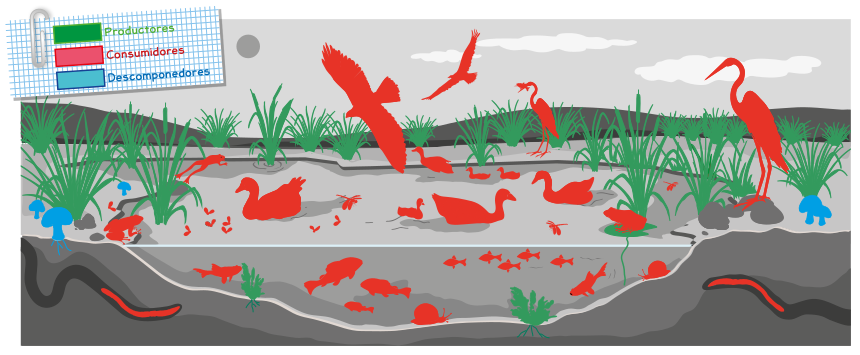
\includegraphics[width=0.8\linewidth]{Tema1/21_Relaciones_alimentarias.png}
    \caption{Relaciones alimentarias en el ecosistema}
    \label{fig:relaciones-alimentarias-ecosistema}
\end{figure}

\subsection{Cadenas y redes tróficas}

Las relaciones tróficas de un ecosistema pueden representarse con unos esquemas llamados \textbf{cadenas y redes tróficas} (Figura: \ref{fig:cadenas-redes-troficas}) en los que se indica, mediante flechas, cómo circula el alimento entre un grupo de seres del ecosistema. Las flechas de estos gráficos siempre apuntan hacia el ser vivo que obtiene el alimento.
\begin{itemize}
    \item \textbf{Las cadenas tróficas.} En una cadena trófica se representa una \textbf{relación lineal de seres vivos} que obtienen su alimento unos de los otros. En ella se parte de un productor, del que se alimenta un consumidor, del que se alimenta otro consumidor...
    \item \textbf{Las redes tróficas.} En las redes tróficas se representan \textbf{varias cadenas tróficas relacionadas}. Se ajustan más a las relaciones tróficas reales del ecosistema, porque reflejan el hecho de que cada tipo de ser vivo puede tener varias fuentes de alimento, o puede servir como alimento a algunos tipos de seres.
\end{itemize}

\begin{figure}[!ht]
    \centering
    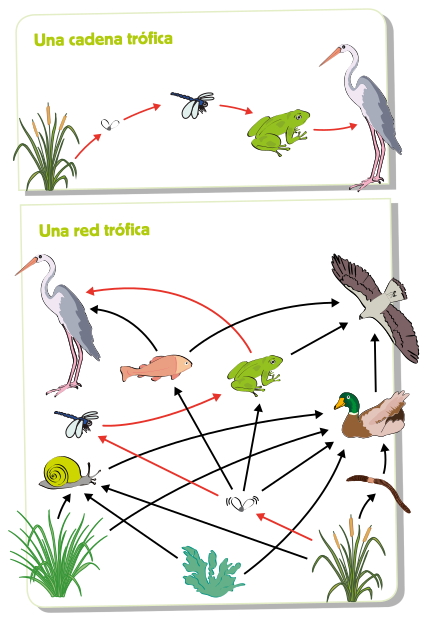
\includegraphics[width=0.4\linewidth]{Tema1/22_Cadenas_Redes_Troficas.png}
    \caption{Cadenas y redes tróficas}
    \label{fig:cadenas-redes-troficas}
\end{figure}

\subsection{Las adaptaciones}

Las especies que forman la biocenosis o comunidad están \textbf{adaptadas} para sobrevivir y reproducirse en el ecosistema del que forman parte. Las \textbf{adaptaciones} son características de estos seres vivos que les permiten:
\begin{itemize}
    \item \textbf{Aprovechar o soportar las condiciones del biotopo}: obtener oxígeno, conseguir agua, desplazarse, resistir el clima...
    \item \textbf{Relacionarse con otros seres vivos}: alimentarse, defenderse, asociarse, aparearse...
\end{itemize}
Las adaptaciones pueden ser partes u órganos del cuerpo de los seres vivos; por ejemplo, las aletas o las branquias de los animales acuáticos o el tallo que almacena agua en los cactus. También pueden ser características del funcionamiento o del comportamiento de los seres vivos, como la pérdida de la hoja de los robles en otoño, los cantos de cortejo de las aves...

\subsection{El ser humano y los ecosistemas}

Como los demás seres vivos, las personas formamos parte de ecosistemas. Nuestra principal adaptación, nuestra inteligencia, nos hace capaces de integrarnos y prosperar en casi todos los ecosistemas del planeta. Somos consumidores muy eficaces, ya que obtenemos alimentos de otros seres vivos que cazamos, recolectamos, criamos o cultivamos. Pero además, de los ecosistemas obtenemos materiales, agua, aire, energía, espacio...

\vspace{3mm}
Por estas razones, nos hemos extendido por casi todo el planeta y hemos tenido gran éxito. Pero nuestra presencia está produciendo daños y desequilibrios en muchos ecosistemas. Los principales son los siguientes:
\begin{itemize}
    \item \textbf{El agotamiento de los recursos}. Consumimos tantos recursos y tan rápido que no da tiempo a que se regeneren de forma natural. Así, por ejemplo:
    \begin{itemize}
        \item Estamos agotando recursos como el petróleo, los minerales o el agua dulce.
        \item Estamos poniendo en \textbf{peligro de extinción} a muchos seres vivos que recolectamos o capturamos en exceso y no tienen tiempo de recuperarse mediante la reproducción.
    \end{itemize}
    \item \textbf{La alteración o destrucción de ecosistemas}. Nuestras actividades hacen que los ecosistemas se alteren o incluso se destruyan, con la consiguiente extinción de muchos de los seres que contienen. Las principales causas son:
    \begin{itemize}
        \item La \textbf{contaminación} del aire, del agua o del suelo con sustancias perjudiciales.
        \item La \textbf{acumulación de residuos} tanto en medios terrestres como acuáticos.
        \item La \textbf{ocupación del territorio} con cultivos, pastos, poblaciones, instalaciones...
        \item La \textbf{introducción de especies} en ecosistemas que no son los suyos. Estas especies provocan graves desequilibrios en esos ecosistemas.
    \end{itemize}
\end{itemize}

\chapter{Relieve e hidrografía de España y de Europa}

\begin{figure}[ht]
    \centering
    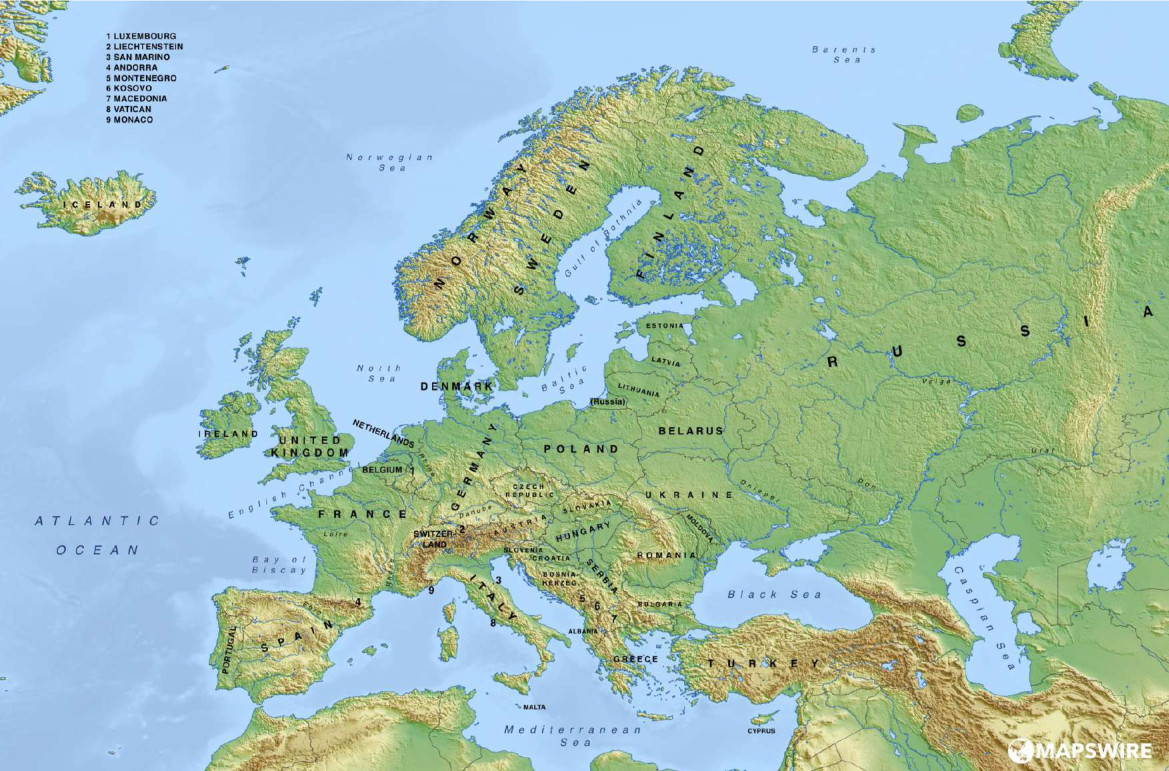
\includegraphics[width=1\linewidth]{Tema2/01_mapa_europa_fisico.jpg}
    \caption{Mapa físico de Europa}
    \label{fig:mapa-fisico-europa}
\end{figure}

\include{Tema2S01_Situacion_y_relieve_de_España}
\section{La situación y el relieve de Europa}

Europa es un continente pequeño por su extensión. Está situado en el hemisferio norte de la Tierra. Está entre los océanos Glacial Ártico y Atlántico, y entre los continentes de Asia y África. Sus límites son el océano Glacial Ártico, al norte; el mar Mediterráneo, al sur; los montes Urales, el mar Caspio, el Cáucaso y el mar Negro, al este; y el océano Atlántico, al oeste.

\subsection{El relieve}

\subsubsection{El relieve de interior: llanuras, montañas antiguas y montañas jóvenes}

\begin{itemize}
    \item Las \textbf{llanuras} se encuentran en el centro del continente y destaca la Gran Llanura Europea.
    \item Las \textbf{mesetas} y las \textbf{montañas antiguas} poco elevadas y de formas redondeadas se encuentran en el norte y en el centro del continente. Destacan el macizo Central francés, los Montes Escandinavos y los montes Urales.
    \item Las \textbf{montañas jóvenes} de gran altura se localizan en el sur del continente. Las más importantes son los Pirineos, los Alpes, los Apeninos, los Cárpatos y el Cáucaso.
\end{itemize}

\subsubsection{El relieve de costa}

Las costas de Europa son muy recortadas, debido a que abundan penínsulas, como la ibérica, la itálica…; cabos, como Norte, Fisterra...; y golfos, como Génova, Bizkaia, Botnia... También pertenecen al continente europeo muchas islas:
\begin{itemize}
    \item En el océano Atlántico se localizan las islas de Islandia, Irlanda, Gran Bretaña, Azores, Madeira, el archipiélago de Canarias, etc.
    \item En el mar Mediterráneo se encuentran las islas de Córcega, Cerdeña, Sicilia, Malta, Creta y Chipre, el archipiélago de Baleares, etc.
\end{itemize}

\subsection{La modificación del relieve}

El relieve, tanto de interior como de costa, sufre modificaciones debido a causas internas y externas. Las \textbf{causas internas} (Figura \ref{fig:causas-internas}) provocan el levantamiento, el hundimiento o el desplazamiento del terreno. En ocasiones, se manifiestan de forma violenta produciendo catástrofes naturales. Destacan los terremotos, los tsunamis, o terremotos submarinos, y los volcanes. Las \textbf{causas externas} (Figura \ref{fig:causas-externas}) desgastan el relieve, transportan los materiales y los depositan en ciertas áreas. Los principales agentes externos son la atmósfera, el agua y los seres vivos.

\begin{figure}[!ht]
    \centering
    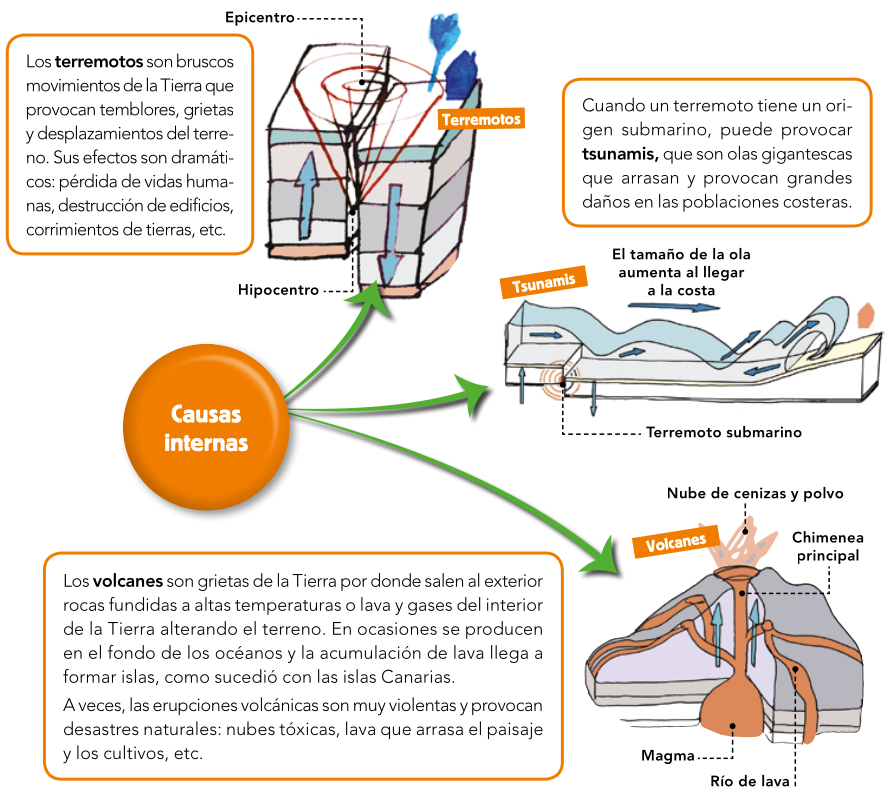
\includegraphics[width=0.7\linewidth]{Tema2/05_causas_internas.png}
    \caption{Causas internas de la modificación del relieve}
    \label{fig:causas-internas}
\end{figure}

\begin{figure}[!ht]
    \centering
    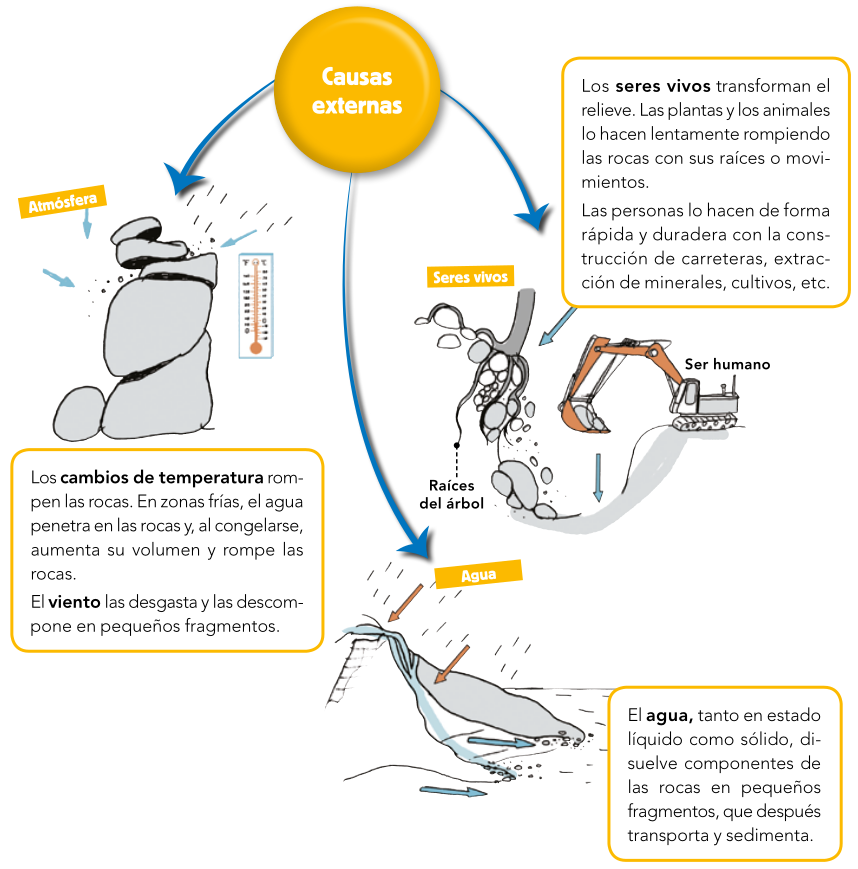
\includegraphics[width=0.7\linewidth]{Tema2/06_causas_externas.png}
    \caption{Causas externas de la modificación del relieve}
    \label{fig:causas-externas}
\end{figure}
\section{La hidrosfera: las aguas del planeta}

\subsection{La hidrosfera y su distribución}

La \textbf{hidrosfera} es el conjunto de todas las aguas de la Tierra: océanos, mares, ríos, lagos, glaciares, aguas subterráneas y vapor de agua. Cubre, aproximadamente, el 70 \% de la superficie terrestre. El agua es una sustancia que puede encontrarse en la naturaleza en tres estados: líquido, hielo y vapor de agua. El agua en la Tierra está distribuida de la siguiente forma: el 97,5 \% es salada (mares y océanos) y solo el 2,5 \% es dulce.

\subsection{La hidrosfera y su clasificación}

Las aguas de la hidrosfera están presentes en dos conjuntos: aguas superficiales y aguas subterráneas.

\vspace{3mm}
\textbf{Las aguas superficiales}

\vspace{3mm}
Estas aguas se encuentran sobre la superficie de la corteza terrestre. Se distinguen dos grandes grupos:
\begin{itemize}
    \item \textbf{Aguas marinas}. Están formadas por océanos y mares. Son saladas y cubren gran parte de la superficie terrestre.
    \item \textbf{Aguas continentales}. A este grupo pertenecen ríos, arroyos, lagos, lagunas, masas de hielo de los polos, nieve... Suelen ser dulces.
\end{itemize}

\textbf{Las aguas subterráneas}

\vspace{3mm}
Se forman cuando las aguas superficiales y el agua de lluvia se filtran a través del suelo y se almacenan en el interior de la Tierra en depósitos denominados acuíferos. A veces, cuando circulan bajo la tierra, forman cuevas y galerías. En algunos lugares salen a la superficie, en forma de fuentes o manantiales. En otras ocasiones, se accede a ellas mediante la excavación de pozos.

\subsection{La importancia de la hidrosfera}

El agua de la hidrosfera es fundamental para el ser humano y el resto de los seres vivos, ya que:
\begin{itemize}
    \item Contribuye a mantener templada la Tierra porque absorbe el calor del Sol.
    \item Es el medio en el que viven los seres acuáticos.
    \item Los seres vivos la necesitamos: las plantas, para fabricar su alimento en la fotosíntesis; los animales, para el funcionamiento del cuerpo.
    \item Los seres humanos la utilizamos para las industrias, la limpieza, el ocio, los transportes, etcétera.
\end{itemize}
\section{Las aguas continentales}

\subsection{Los ríos}

Los ríos son corrientes naturales y continuas de agua dulce que nacen en zonas montañosas, atraviesan valles y llanuras y desembocan en el mar, en un lago o en otro río. Los ríos que desembocan en otro se denominan afluentes.

\vspace{3mm}
\textbf{Principales elementos de un río} (Figura: \ref{fig:elementos-rio})
\begin{itemize}
    \item \textbf{Nacimiento} es el lugar donde nace o brota.
    \item \textbf{Curso} es el recorrido desde su nacimiento hasta la desembocadura. Se diferencian tres partes:
    \begin{itemize}
        \item \textbf{Curso alto} es el tramo más cercano a su nacimiento. En este tramo, las aguas corren rápidas y arrastran gran cantidad de arena y piedras, produciendo una gran erosión.
        \item \textbf{Curso medio} es el tramo entre el curso alto y el curso bajo. Alterna zonas de fuerte erosión con zonas donde se depositan la arena y las piedras debido a los cambios de la pendiente.
        \item \textbf{Curso bajo} es el tramo próximo a la desembocadura. En esta zona, la pendiente es casi nula y presenta meandros o grandes curvaturas. Debido a la acumulación de los materiales en este tramo se forman deltas y estuarios.
    \end{itemize}
    \item \textbf{Cauce} es el terreno por donde discurren las aguas del río.
\end{itemize}

\begin{figure}[!ht]
    \centering
    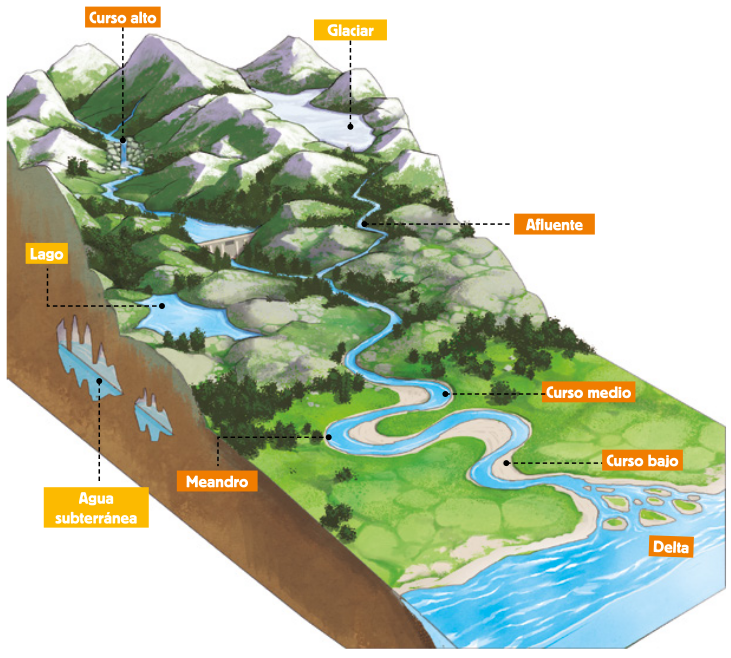
\includegraphics[width=0.7\linewidth]{Tema2/07_Aguas_continentales.png}
    \caption{Elementos de un río}
    \label{fig:elementos-rio}
\end{figure}

\textbf{Principales características de un río}

\begin{itemize}
    \item \textbf{Longitud} es la distancia entre su nacimiento y la desembocadura.
    \item \textbf{Caudal} es la cantidad de agua que lleva un río en un lugar y momento determinado.
    \item \textbf{Régimen} es la variación de caudal a lo largo del año. Es regular cuando no varía a lo largo del año, e irregular, cuando sufre grandes crecidas en épocas de lluvia y está casi seco durante el resto del año.
\end{itemize}
Estas características diferencian a un río de otro, debido principalmente a dos factores: el relieve y el clima.
\begin{itemize}
    \item El \textbf{relieve} influye en la longitud y la velocidad de las aguas del río. Los ríos son más largos cuanto más alejadas están las montañas donde nacen del mar en que desembocan.
    \item El \textbf{clima} repercute en el caudal y el régimen de los ríos. Así, los ríos que atraviesan zonas lluviosas son muy caudalosos y tienen régimen regular. Sin embargo, los ríos que discurren por zonas con climas secos tienen un régimen irregular.
\end{itemize}

\subsection{Otras aguas}

\begin{itemize}
    \item \textbf{Glaciares}

    Son grandes acumulaciones de hielo. Se encuentran en los polos y en la alta montaña.
    \item \textbf{Lagos}
    
    Son acumulaciones de agua en depresiones del relieve. Cuando estas son más pequeñas se llaman lagunas.
    \item \textbf{Acuíferos}

    Son acumulaciones de agua subterránea. Se forman por las filtraciones de agua desde la superficie terrestre.
\end{itemize}
\include{Tema2S05_Hidrografia_España}
\section{La hidrografía de Andalucía}

\subsection{Los ríos andaluces}

Los ríos de nuestra comunidad (Figura \ref{fig:rios-andaluces}) son cortos, poco caudalosos y de régimen irregular. Unos desembocan en el océano Atlántico, y otros, en el mar Mediterráneo.

\begin{figure}[!ht]
    \centering
    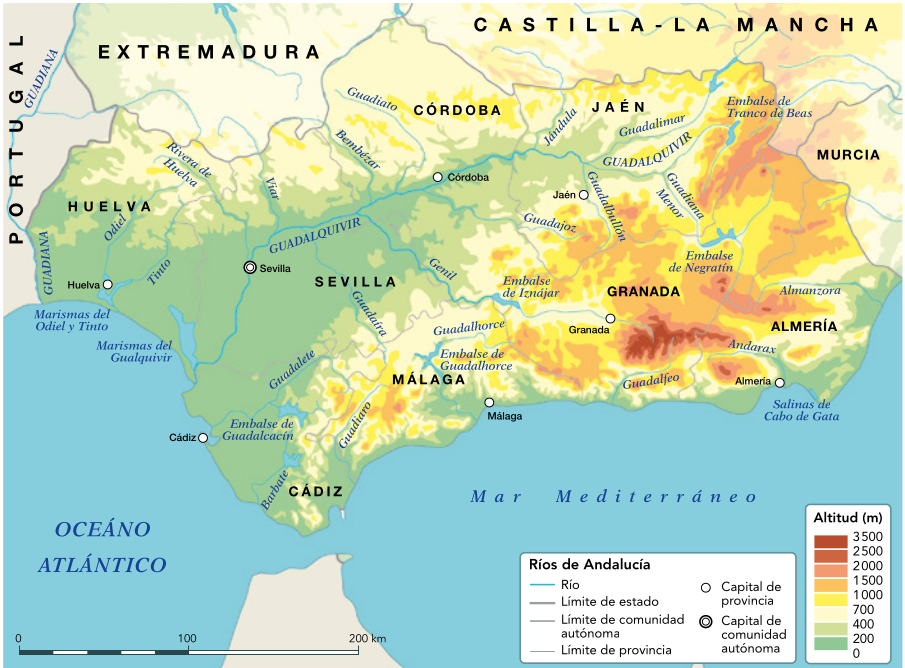
\includegraphics[width=1\linewidth]{Tema2/09_Rios_andaluces.png}
    \caption{Ríos andaluces}
    \label{fig:rios-andaluces}
\end{figure}

\subsubsection{Los ríos de la vertiente atlántica}

Los ríos de esta vertiente son los más largos y caudalosos de la comunidad, su régimen es irregular. Destacan el Barbate, el Tinto, el Odiel, el Guadalete, el Guadiana y el Guadalquivir.

\begin{itemize}
    \item El \textbf{Guadiana} nace en la provincia de Ciudad Real y desemboca en Ayamonte (Huelva), formando frontera con Portugal.
    \item El \textbf{Guadalquivir} es el río más largo e importante de Andalucía. Nace en la sierra de Cazorla, en la Cañada de las Fuentes, en Quesada (Jaén). Atraviesa las provincias de Jaén, Córdoba, Sevilla, desde donde es navegable hasta su desembocadura, en Sanlúcar de Barrameda (Cádiz), tras recorrer 580 km. Sus principales afluentes son el Guadiamar, el Jándula, el Genil, el Guadiana Menor y el Guadajoz.
\end{itemize}

En muchos de estos ríos se han construido embalses, como el de Tranco de Beas, en el Guadalquivir, y el de Iznájar, en el Genil.

\subsubsection{Los ríos de la vertiente mediterránea}

Los ríos que desembocan en el Mediterráneo nacen en la cordillera Penibética. Son \textbf{ríos cortos} y su \textbf{caudal es escaso y muy irregular}. Los más importantes son el Guadiaro, el Guadalhorce, el Guadalfeo, el Andarax y el Almanzora. En estos ríos hay embalses, como el de Negratín, en el Guadiana Menor, y el embalse de Guadalhorce.

\subsection{Las lagunas y los humedales}

Andalucía cuenta con un \textbf{gran número de lagunas y humedales}, que conforman ecosistemas en el que conviven especies protegidas tanto de flora como de fauna. El origen de estos ecosistemas es muy variado:

\begin{itemize}
    \item Sin salida al mar, como las lagunas de Zóñar y Tíscar en Córdoba, de Fuente de Piedra en Málaga y Salinas de Cabo de Gata en Almería.
    \item Creados por la intervención humana, como Laguna Grande en Jaén o el embalse de Malpasillo y Cordobilla, entre las provincias de Córdoba y Sevilla.
    \item \textbf{Marismas}, formadas en la desembocadura de los ríos Odiel y Tinto en Huelva y en la del río Guadalquivir en Sanlúcar de Barrameda (Cádiz). Estas marismas se adentran hasta varios municipios de la provincia de Sevilla, formando parte del Parque Natural de Doñana.
\end{itemize}
\section{La hidrografía de Europa}

\begin{figure}[!ht]
    \centering
    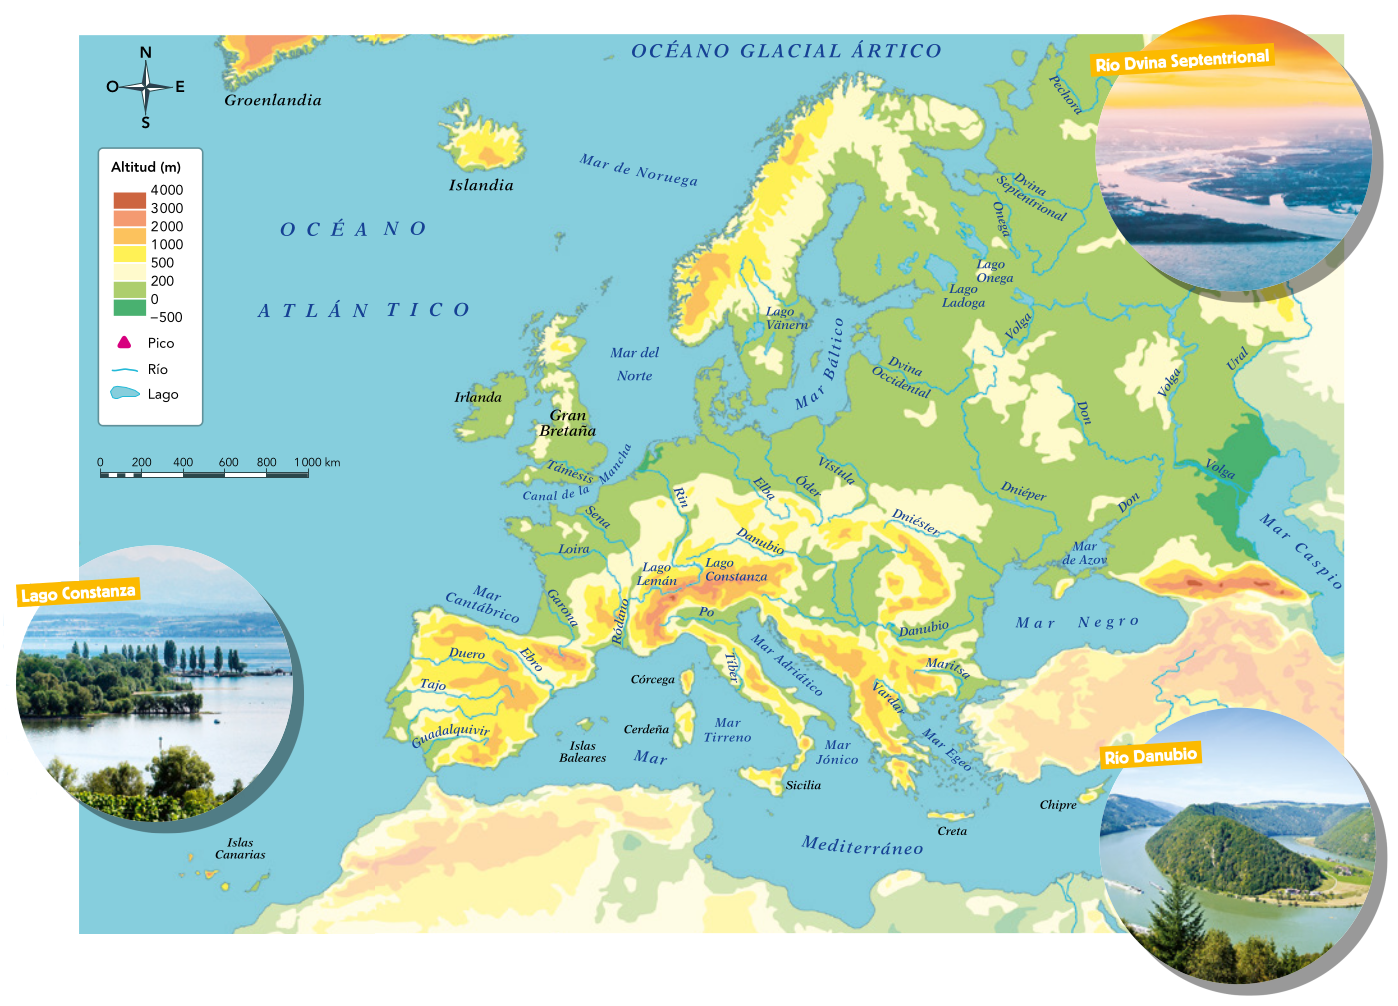
\includegraphics[width=1\linewidth]{Tema2/10_Rios_Europa.png}
    \caption{Hidrografía de Europa}
    \label{fig:hidrografia-europa}
\end{figure}

\subsection{Los océanos y los mares}

Europa está rodeada de océanos y mares. En las costas del norte y el oeste del continente, tenemos los océanos Glacial Ártico y Atlántico.

\vspace{3mm}
Los mares que bañan las costas de Europa son el de Noruega, del Norte, Báltico, Cantábrico, el Mediterráneo, el Adriático, etcétera. También hay dos mares interiores, el mar Negro y el mar Caspio.

\subsection{Los lagos europeos}

Los lagos en Europa son muy abundantes.

\begin{enumerate}
    \item En el norte destacan el Ladoga y el Onega.
    \item Los lagos centroeuropeos como el Lemán y el Constanza se encuentran a lo largo de los Alpes.
    \item Los lagos mediterráneos son de menor tamaño.
\end{enumerate}

\subsection{Los ríos europeos}

Las características de los ríos europeos están determinadas por el relieve y el clima.

\subsubsection{Los ríos de las vertientes ártica y atlántica}

Son ríos largos que suelen tener cuencas muy extensas.

\begin{itemize}
    \item Los ríos que desembocan en el Glacial Ártico son caudalosos e irregulares, como el Dvina Septentrional.
    \item Los ríos que desembocan en el océano Atlántico son caudalosos y regulares. Destacan el Vístula, el Rin, el Sena y el Loira.
\end{itemize}

\subsubsection{Los ríos de la vertiente mediterránea}

Estos suelen ser cortos e irregulares, como el Po.

\subsubsection{Los ríos que desembocan en los mares interiores}

Estos ríos son largos, caudalosos y navegables. Destaca el Danubio, que vierte sus aguas en el mar Negro y el Volga, que es el río más largo de Europa y desemboca en el mar Caspio.
\section{Utilización y conservación: consumo responsable}

\subsection{El agua, un recurso imprescindible}

El agua es un recurso imprescindible para la vida, ya que ningún ser vivo puede sobrevivir sin ella. El agua es un bien escaso y su disponibilidad está relacionada con la calidad de vida. Sin embargo, no todas las personas tienen acceso a ella de la misma manera. Para hacer un uso responsable del agua, tenemos que tener en cuenta los datos siguientes:

\begin{enumerate}
    \item Unos 663 millones de personas no tienen acceso a agua potable, lo que supone un riesgo para la salud.
    \item El 97,5 \% del agua de la Tierra es agua salada, mientras que el resto, un 2,5 \%, es agua dulce.
    \item Cada 20 segundos fallece un niño o una niña menor de 5 años como consecuencia del consumo de agua no potable y malnutrición.
    \item Las familias en los países subdesarrollados emplean diariamente unas cinco horas para acceder al agua.
\end{enumerate}

\subsection{Medidas de ahorro y consumo responsable}

En los países desarrollados, el agua está presente en muchas de las actividades que se realizan diariamente en el hogar (aseo, higiene, limpieza...), en las localidades (limpieza, riego...), en la agricultura y ganadería, en la industria, en el ocio...

\vspace{3mm}
El uso, a veces, descontrolado que hace el ser humano del agua así como las condiciones climáticas, como la escasez de precipitaciones, hace que este recurso natural se agote.

\vspace{3mm}
Por ese motivo, es responsabilidad de todas las personas controlar ese consumo tomando medidas eficientes y responsables para asegurar el abastecimiento presente y futuro de agua potable. Así se contribuye a la mejora del medio ambiente y al ahorro en la factura del agua.

\subsection{Algunas medidas para el ahorro del agua}

\begin{figure}[!ht]
    \centering
    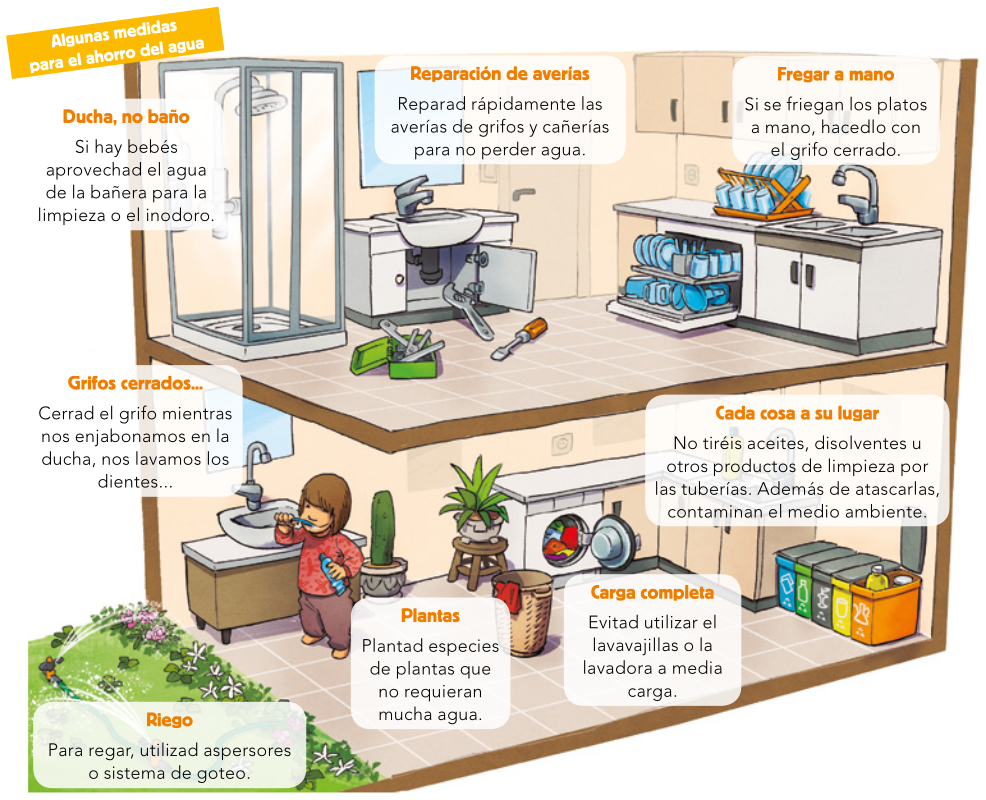
\includegraphics[width=1\linewidth]{Tema2/11_Medidas_ahorro_agua.png}
    \caption{Medidas para el ahorro del agua}
    \label{fig:medidas-ahorro-agua}
\end{figure}


\addcontentsline{toc}{chapter}{TRIMESTRE 2}
\part*{Trimestre 2}

\chapter{Las funciones vitales}

\begin{figure}[ht]
    \centering
    
\includegraphics[width=1\linewidth]{Tema3/00_Vida.png}
    \caption{Las funciones vitales}
    \label{fig:funciones-vitales}
\end{figure}

\section{La función de nutrición}

Mediante la función de nutrición, tomamos alimentos y agua, respiramos oxígeno, utilizamos estas sustancias para vivir y crecer, y expulsamos los desechos.

\vspace{3mm}
Para realizar esta función, trabajan coordinadamente cuatro aparatos: el \textbf{digestivo}, el \textbf{respiratorio}, el \textbf{circulatorio} y el \textbf{excretor}.

\subsection{Los nutrientes y los alimentos}

\subsubsection{Los nutrientes}

Los nutrientes son todas aquellas sustancias que obtenemos de los alimentos y que necesitan las células de nuestro cuerpo para realizar sus funciones vitales. Los principales nutrientes son:

\begin{itemize}
    \item Los \textbf{hidratos de carbono} o azúcares proporcionan energía.
    \item Los \textbf{lípidos} pueden ser de distintos tipos, y cumplen diversas funciones. Por ejemplo, las grasas proporcionan energía; pueden ser almacenadas en algunas células de la piel como una reserva energética que, además, nos aísla del frío.
    \item Las \textbf{proteínas} son imprescindibles para que las células se formen, crezcan y desarrollen tejidos.
    \item Las \textbf{vitaminas} y las \textbf{sales minerales} regulan el funcionamiento general del organismo.
    \item El \textbf{agua} constituye la mayor parte del contenido de las células, de la sangre, etc. Sin ella, no funcionaría el organismo.
\end{itemize}

\subsubsection{Los alimentos}

Según los nutrientes que contienen, los alimentos se clasifican en energéticos, constructivos y reguladores.

\begin{itemize}
    \item Los \textbf{alimentos energéticos} contienen hidratos de carbono o grasas. Son los aceites vegetales, las grasas animales, la mantequilla, las patatas y los cereales y sus derivados, como las pastas, los dulces y el pan.
    \item Los \textbf{alimentos constructivos} contienen proteínas. Son las legumbres, las carnes de animales terrestres o marinos, los huevos y la leche y sus derivados, como los yogures y los quesos.
    \item Los \textbf{alimentos reguladores} contienen vitaminas y sales minerales. Son las verduras, las hortalizas y las frutas.
\end{itemize}

\subsubsection{La dieta y la rueda de los alimentos}

La \textbf{dieta} es el conjunto de los alimentos y el agua que toma cada día una persona. La \textbf{dieta es saludable} cuando contiene una cantidad adecuada de cada uno de los nutrientes.

\vspace{3mm}
Para que resulte más fácil elaborar dietas saludables, los alimentos se representan en la \textbf{rueda de los alimentos} (Figura \ref{fig:rueda-alimentos}), un gráfico que nos orienta sobre la frecuencia con la que se deben consumir los diferentes alimentos.

\begin{figure}[!ht]
    \centering
    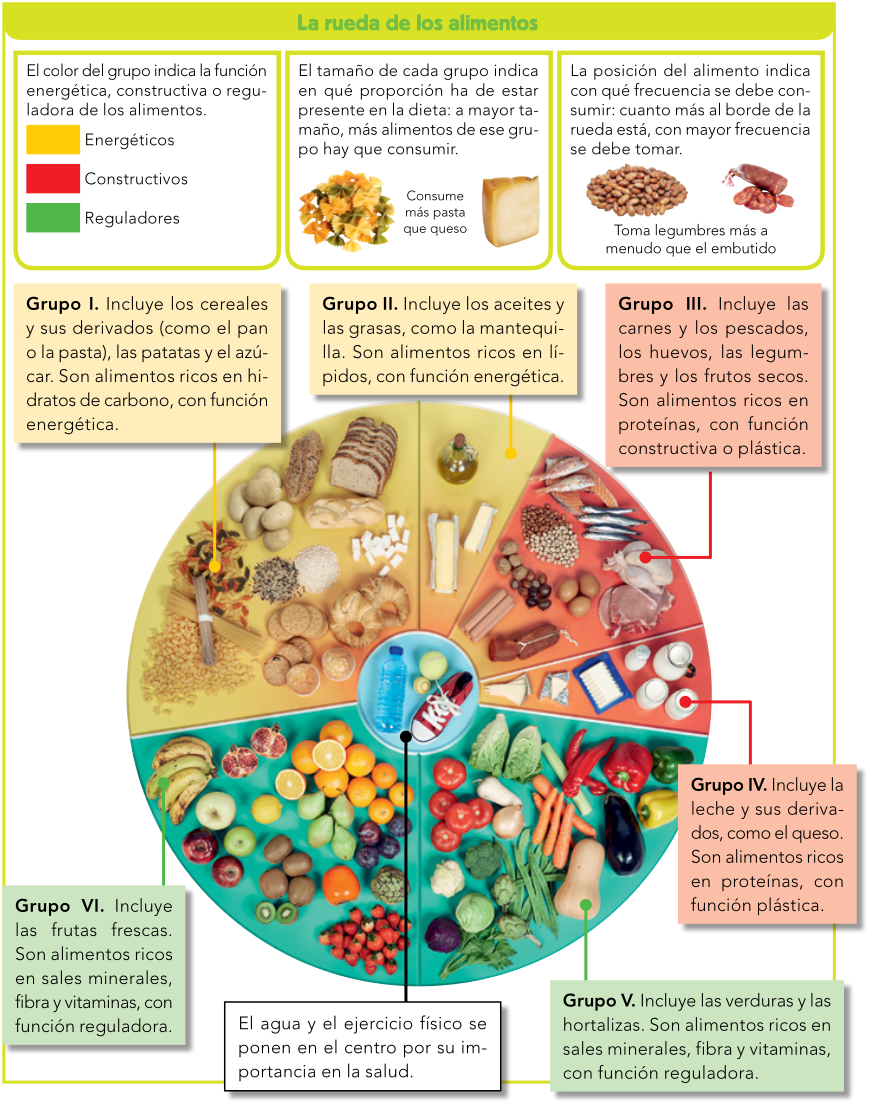
\includegraphics[width=1\linewidth]{Tema3/01_Rueda_alimentos.png}
    \caption{Rueda de los alimentos}
    \label{fig:rueda-alimentos}
\end{figure}

\subsection{El aparato digestivo y la digestión}

Nuestras células necesitan nutrientes y agua para llevar a cabo sus actividades. Estas sustancias las obtenemos de los alimentos y las bebidas mediante la digestión. El aparato encargado de realizar la digestión es el aparato digestivo (Figura \ref{fig:aparato-digestivo}).

\subsubsection{Cómo es el aparato digestivo}

El aparato digestivo está formado por el tubo digestivo y las glándulas anejas.

\begin{itemize}
    \item El \textbf{tubo digestivo} es un largo conducto compuesto por la boca, la faringe, el esófago, el estómago, el intestino delgado, el intestino grueso y el ano.
    \item Las \textbf{glándulas anejas} son órganos que se encuentran fuera del tubo digestivo pero que vierten en él las sustancias que producen. Son las \textbf{glándulas salivales}, el \textbf{hígado} y el \textbf{páncreas}.
\end{itemize}

\begin{figure}[!ht]
    \centering
    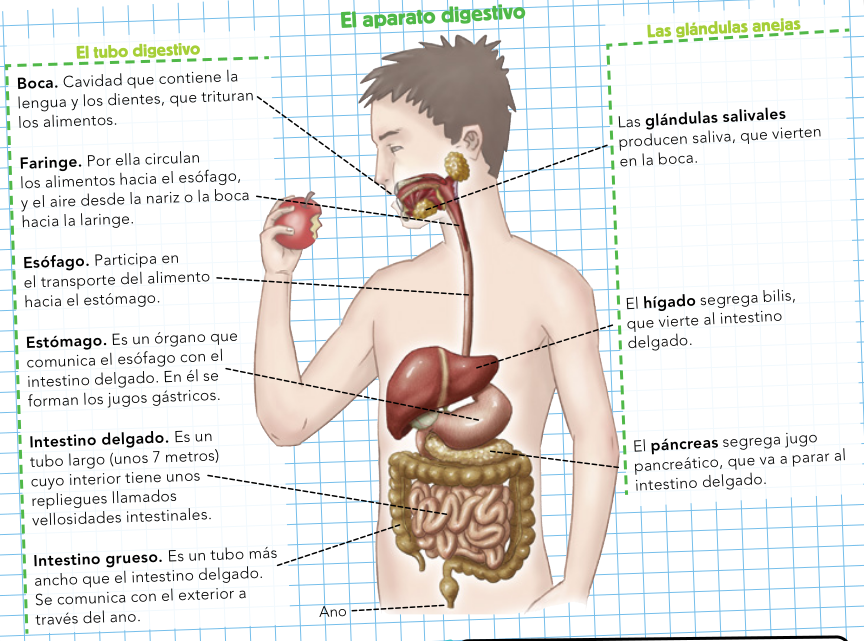
\includegraphics[width=0.8\linewidth]{Tema3/02_Aparato_digestivo.png}
    \caption{El aparato digestivo}
    \label{fig:aparato-digestivo}
\end{figure}

\subsubsection{La digestión}

La \textbf{digestión} (Figura \ref{fig:digestion}) es la transformación de los alimentos que tomamos, para extraer de ellos los nutrientes. Tiene lugar a lo largo del tubo digestivo, y se lleva a cabo en varias etapas.

\vspace{3mm}
\textbf{En la boca}

\vspace{3mm}
En la boca, los dientes y las muelas cortan y trituran los alimentos. Estos se mezclan con la saliva, gracias a los movimientos de la lengua, y se forma el \textbf{bolo alimenticio}. Este, al ser tragado, baja por la faringe y el esófago hasta el estómago.

\vspace{3mm}
\textbf{En el estómago}

\vspace{3mm}
Cuando llega el bolo alimenticio al estómago, sus paredes segregan unas sustancias, los jugos gástricos, que digieren parcialmente el alimento y lo transforman en una papilla, llamada \textbf{quimo}.

\vspace{3mm}
\textbf{En el intestino delgado}

\vspace{3mm}
Cuando el quimo llega al intestino delgado, se vierten en él el jugo pancreático (procedente del páncreas) y la bilis (procedente del hígado). Se completa así la digestión de los alimentos y el quimo se transforma en el \textbf{quilo}.

\vspace{3mm}
A continuación, los nutrientes del quilo pasan a la sangre a través de los capilares que se encuentran en el intestino delgado, este proceso se llama \textbf{absorción}.

\vspace{3mm}
\textbf{En el intestino grueso}

\vspace{3mm}
El agua y los desechos pasan al intestino grueso. Allí se reabsorbe el agua de la mezcla y se forman las \textbf{heces}, sustancias de desecho que son expulsadas por el ano.

\begin{figure}[!ht]
    \centering
    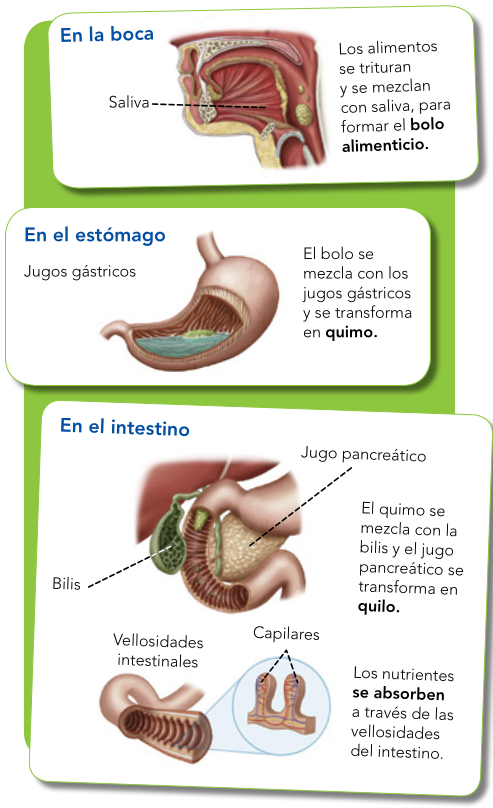
\includegraphics[width=0.7\linewidth]{Tema3/03_Digestion.png}
    \caption{La digestión}
    \label{fig:digestion}
\end{figure}

\subsection{El aparato respiratorio y la respiración}

\subsubsection{Las células necesitan oxígeno}

Mediante la respiración, obtenemos del aire el oxígeno que necesitan nuestras células y expulsamos al exterior el dióxido de carbono que estas producen como desecho. De este proceso se encarga el aparato respiratorio.

\subsubsection{El aparato respiratorio}

El aparato respiratorio (Figura \ref{fig:aparato-respiratorio}) está formado por las vías respiratorias y por los pulmones.

\vspace{3mm}
\textbf{Las vías respiratorias}

\vspace{3mm}
Las vías respiratorias son tubos que conectan los pulmones con el exterior. Son las \textbf{fosas nasales}, la \textbf{faringe}, la \textbf{laringe}, la \textbf{tráquea} y los \textbf{bronquios}.

\vspace{3mm}
\textbf{Los pulmones}

\vspace{3mm}
Los pulmones son dos órganos esponjosos situados en el tórax y separados del abdomen por un músculo, el \textbf{diafragma}. Están formados por las ramificaciones de los \textbf{bronquios} y por los \textbf{alvéolos}.

\begin{figure}[!ht]
    \centering
    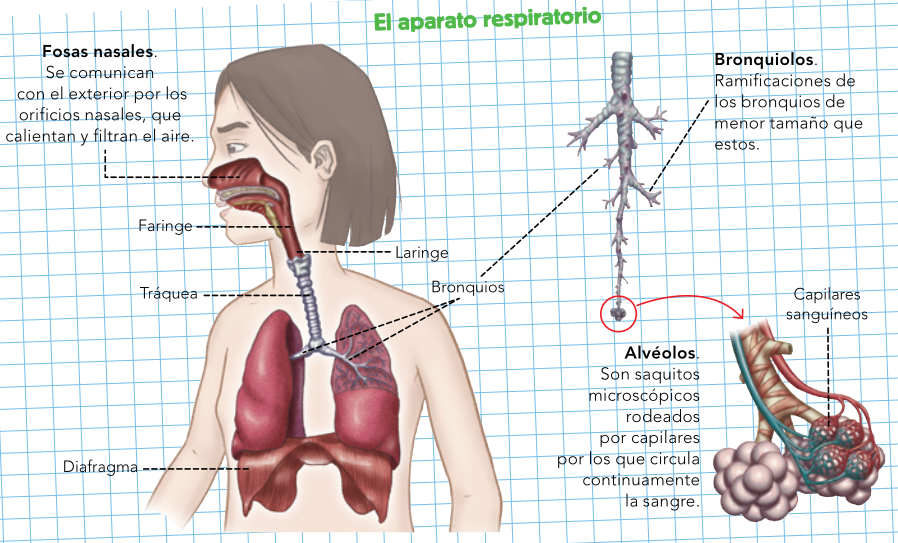
\includegraphics[width=0.9\linewidth]{Tema3/04_Aparato_respiratorio.png}
    \caption{Aparato respiratorio}
    \label{fig:aparato-respiratorio}
\end{figure}

\subsubsection{La respiración}

El aparato respiratorio realiza su función en tres etapas (Figura \ref{fig:respiracion}): la inspiración (o entrada de aire que contiene oxígeno), el intercambio de gases (que sucede en los alvéolos) y la espiración (o expulsión de aire que contiene dióxido de carbono).

\begin{figure}[!ht]
    \centering
    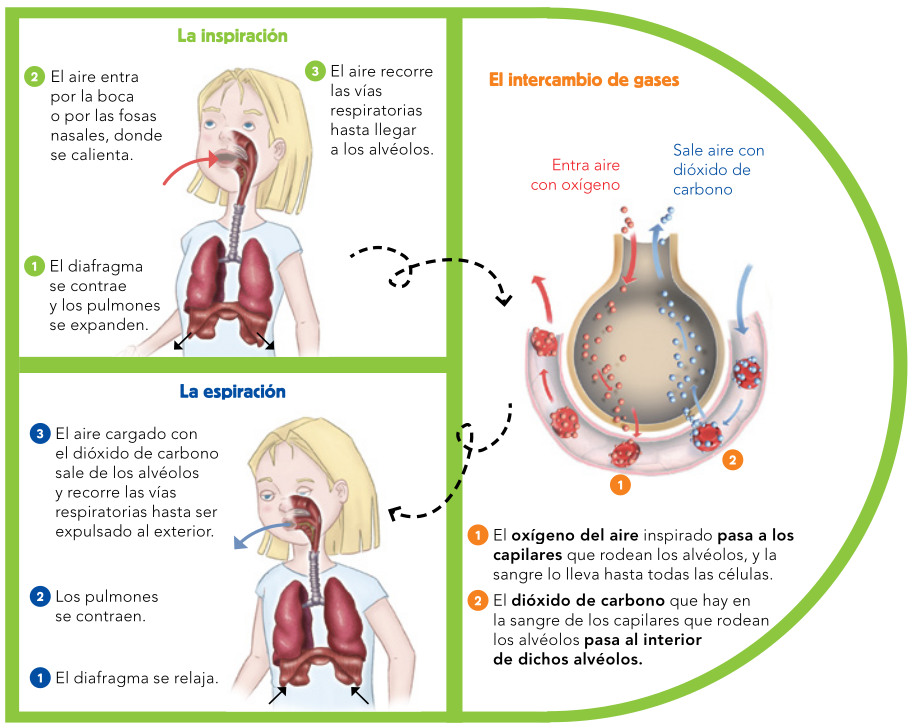
\includegraphics[width=1\linewidth]{Tema3/05_Respiracion.png}
    \caption{La respiración}
    \label{fig:respiracion}
\end{figure}

\subsection{El aparato circulatorio y la circulación}

Las células de nuestro cuerpo necesitan recibir los nutrientes procedentes del aparato digestivo y el oxígeno que llega a través del aparato respiratorio. Además, las células producen desechos, como dióxido de carbono y otras sustancias que hay que llevar hasta los órganos que las eliminan.

\vspace{3mm}
El oxígeno, los nutrientes y los desechos viajan con la sangre de unas partes del cuerpo a otras a través del aparato circulatorio.

\subsubsection{El aparato circulatorio}

El aparato circulatorio está formado por el \textbf{corazón} y por los \textbf{vasos sanguíneos}.

\begin{itemize}
    \item El \textbf{corazón} (Figura \ref{fig:corazon}) es un órgano hueco y musculoso del tamaño de nuestro puño. Está dividido en dos mitades, la izquierda y la derecha, separadas entre sí. En cada mitad hay una cavidad superior, llamada \textbf{aurícula}, y otra inferior, llamada \textbf{ventrículo}; entre ellas hay una \textbf{válvula}, una especie de ``puerta'', que se abre para dejar pasar la sangre en una dirección y se cierra para que esta no vuelva atrás.
    \begin{figure}[!ht]
        \centering
        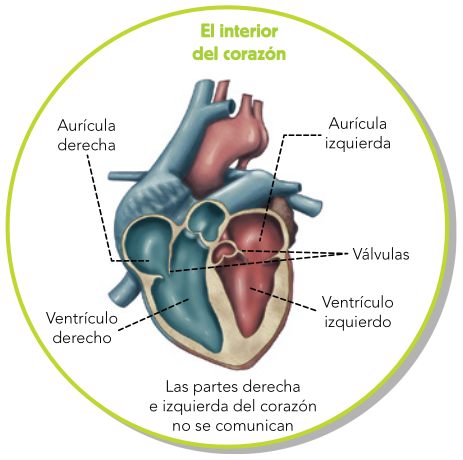
\includegraphics[width=0.6\linewidth]{Tema3/06_Corazon.png}
        \caption{El corazón}
        \label{fig:corazon}
    \end{figure}
    \item Los \textbf{vasos sanguíneos} (Figura \ref{fig:vasos-sanguineos}) son una red de conductos por los que circula la sangre. Son de tres tipos: \textbf{arterias}, \textbf{venas} y \textbf{capilares}.
    \begin{figure}[!ht]
        \centering
        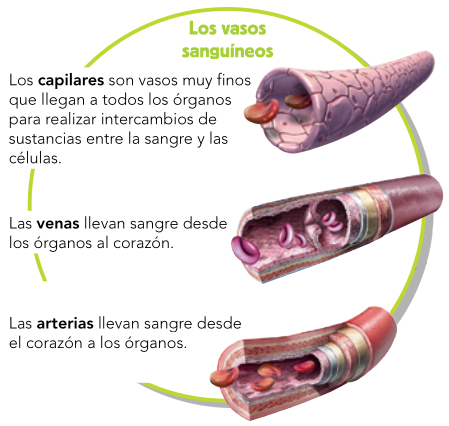
\includegraphics[width=0.7\linewidth]{Tema3/07_Vasos_sanguineos.png}
        \caption{Vasos sanguíneos}
        \label{fig:vasos-sanguineos}
    \end{figure}
\end{itemize}

\subsubsection{La circulación}

La circulación (Figura \ref{fig:circulacion}) se puede dividir en \textbf{circulación pulmonar} y circulación \textbf{general}.

\begin{figure}[!ht]
    \centering
    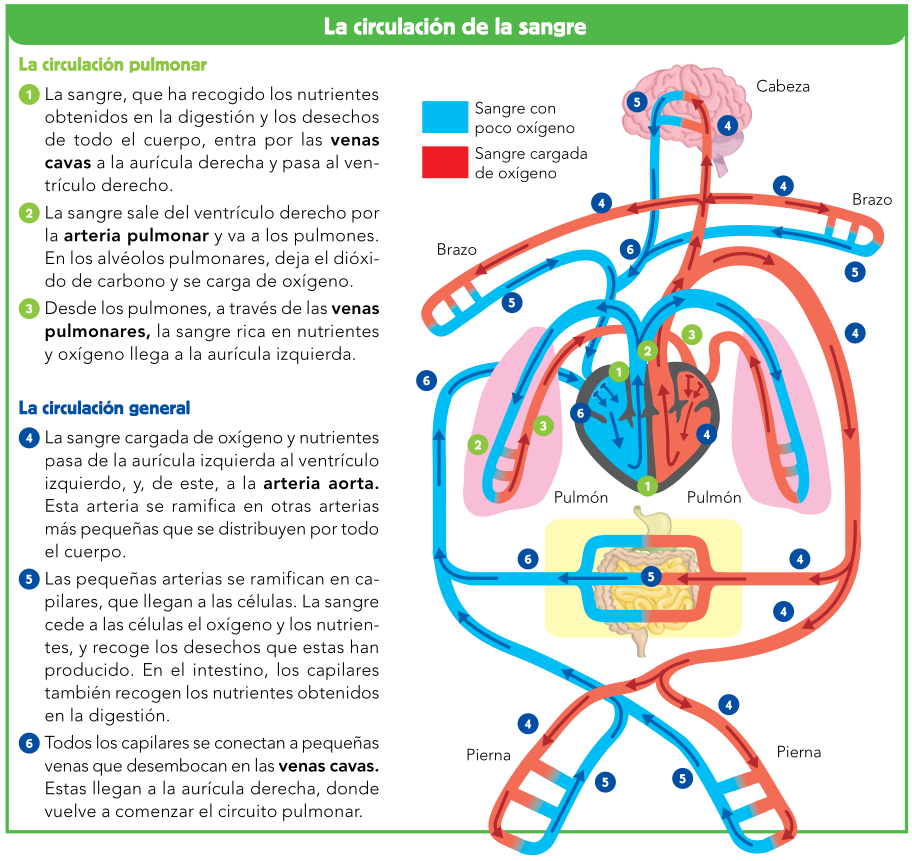
\includegraphics[width=1\linewidth]{Tema3/08_Circulacion.png}
    \caption{La circulación de la sangre}
    \label{fig:circulacion}
\end{figure}

\subsection{La excreción}

La \textbf{excreción} es la expulsión al exterior del cuerpo de las sustancias de desecho que se producen en las 
células.

\vspace{3mm}
Además del dióxido de carbono, que se expulsa mediante el aparato respiratorio, las células producen otras muchas sustancias de desecho, que expulsamos, en su mayor parte, a través del \textbf{aparato excretor} y mediante las \textbf{glándulas sudoríparas} de la piel.

\subsubsection{El aparato excretor}

El aparato excretor (Figura \ref{fig:aparato-excretor}) lo forman los riñones y las vías urinarias.

\begin{itemize}
    \item Los \textbf{riñones}. Son dos órganos con forma de judía, situados en la zona lumbar. Contienen miles de finísimos tubos en los que se limpia la sangre de las sustancias de desecho y se forma la orina.
    \item Las \textbf{vías urinarias}. Son los conductos por los que la orina circula, se almacena y se expulsa al exterior. Son los uréteres, la vejiga urinaria y la uretra.
\end{itemize}

\begin{figure}[!ht]
    \centering
    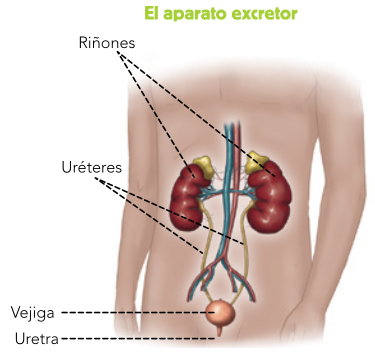
\includegraphics[width=0.7\linewidth]{Tema3/09_Aparato_excretor.png}
    \caption{Aparato excretor}
    \label{fig:aparato-excretor}
\end{figure}

\begin{figure}[!ht]
    \centering
    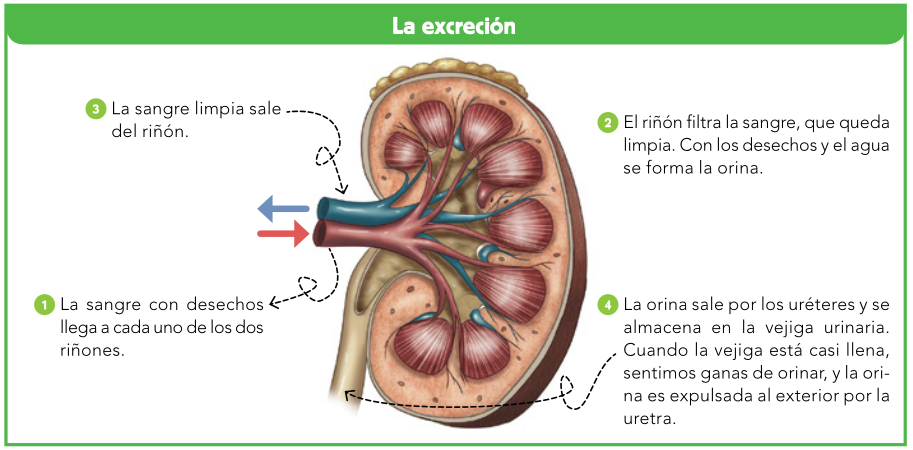
\includegraphics[width=1\linewidth]{Tema3/10_Excrecion.png}
    \caption{La excreción}
    \label{fig:excrecion}
\end{figure}

\subsection{La salud y la emfermedad}

\subsubsection{Qué son la salud y la enfermedad}

La \textbf{salud} es el estado de bienestar desde un punto de vista físico, mental y social. Cuando tenemos salud, nuestro cuerpo funciona bien y nos sentimos a gusto con lo que hacemos, con nuestro ambiente y con los demás.

\vspace{3mm}
La \textbf{enfermedad} es cualquier situación en la que nuestra salud se altera durante un tiempo. Recuerda que una enfermedad se manifiesta con síntomas, que son las señales de que algo no funciona bien en nuestro organismo. Estos síntomas son muy variados y, a partir de ellos, pueden identificarse las enfermedades que podemos sufrir.

\subsubsection{Tipos de enfermedades}

Dependiendo de qué las produce, las enfermedades se pueden clasificar en dos tipos:

\begin{itemize}
    \item Las \textbf{enfermedades infecciosas}. Son las producidas por seres microscópicos, como bacterias o virus, que entran en nuestro cuerpo y nos perjudican. Estos seres llegan a nuestro organismo de varias formas: a través de heridas, picaduras, por el aire que respiramos, por la boca al tomar alimentos en mal estado o sin lavar, al comer con las manos sucias, o al compartir vasos con personas que padecen enfermedades infecciosas… Son enfermedades infecciosas los resfriados, la varicela, la gripe, etc.
    \item Las \textbf{enfermedades no infecciosas}. Son las que se producen por otras causas distintas de los microbios. Por ejemplo: la obesidad, que puede estar provocada por una mala alimentación; las originadas por accidentes, como los cortes, las roturas de huesos, etc.; las causadas por sustancias tóxicas (intoxicaciones); el agotamiento físico y mental provocado por descansar y dormir poco.
\end{itemize}

\subsubsection{Nutrición y salud}

Prevenir es aplicar medidas y hábitos saludables que disminuyen el riesgo de padecer ciertas enfermedades. La prevención se consigue llevando una serie de \textbf{hábitos saludables} para cuidar nuestro organismo. También, acudiendo a \textbf{revisiones médicas} cada cierto tiempo, para detectar si algo funciona mal en nuestro cuerpo y tratarlo antes de que la enfermedad se haga más grave.

\vspace{3mm}
\textbf{Hábitos saludables y nutrición}

\vspace{3mm}
Muchas enfermedades que afectan a los aparatos que intervienen en la nutrición pueden prevenirse siguiendo una serie de hábitos saludables relacionados con el estilo de vida.

\vspace{3mm}
\textbf{Cómo cuidar el aparato digestivo}

\begin{itemize}
    \item Llevar una \textbf{dieta equilibrada} para disminuir el riesgo de enfermedades nutricionales.
    \item \textbf{Tomar fruta y verdura} cada día e incluir en la dieta alimentos que contengan fibra, ya que favorecen el tránsito intestinal.
    \item \textbf{Comer despacio}, masticando bien los alimentos, y tratar de hacer \textbf{cuatro o cinco comidas al día}, preferentemente a las mismas horas.
    \item \textbf{No comer más de lo necesario}, para que tus digestiones sean ligeras.
    \item \textbf{Lavar los alimentos} que tomamos \textbf{y las manos antes y después de comer}, para evitar enfermedades infecciosas e intoxicaciones.
    \item \textbf{Moderar el consumo} de la sal, el chocolate, las salsas picantes, el café, etc., que pueden dañar el aparato digestivo.
    \item Mantener una buena higiene dental lavándote los dientes después de cada comida, para evitar la caries dental.
\end{itemize}

\textbf{Cómo cuidar el aparato respiratorio}

\begin{itemize}
    \item Tratar siempre de \textbf{respirar por la nariz} y no por la boca, ya que las fosas nasales retienen las partículas de polvo, y calientan y humedecen el aire antes de entrar en los pulmones.
    \item Hacer \textbf{ejercicio físico cada día}, ya que mejora la ventilación de los pulmones.
    \item \textbf{No fumar}, ya que el consumo de tabaco se relaciona con muchas enfermedades, entre ellas el cáncer de pulmón.
    \item \textbf{Evitar ambientes contaminados}, y con mucho humo que pueden perjudicar a tus pulmones.
    \item \textbf{Practicar ejercicios de respiración} ya que, además de mejorar la oxigenación de nuestro cuerpo, pueden servir como forma de relajación en situaciones estresantes.
\end{itemize}

\textbf{Cómo cuidar el aparato circulatorio}

\begin{itemize}
    \item Llevar una \textbf{dieta equilibrada} y no abusar de las grasas, la bollería industrial y las golosinas, para evitar enfermedades cardiovasculares.
    \item Realizar \textbf{ejercicio físico a diario y evitar el sedentarismo} para prevenir la obesidad y los infartos.
    \item \textbf{Descansar y dormir} entre 8 y 10 horas son indispensables para evitar la fatiga y el cansancio.
    \item \textbf{Evitar el consumo de alcohol y de tabaco}, para evitar el riesgo de sufrir enfermedades cardiovasculares como los infartos.
\end{itemize}

\textbf{Cómo cuidar el aparato excretor}

\begin{itemize}
    \item \textbf{Beber abundante líquido}, preferiblemente agua, para evitar la concentración de la orina y la aparición de cálculos (piedras en los riñones o en la vejiga).
    \item Llevar una \textbf{dieta equilibrada}, sin abusar de alimentos salados que podrían dañar tus riñones.
\end{itemize}
\section{La función de relación humana}

Como el resto de los vertebrados, las personas tenemos una función de relación muy desarrollada (Figura \ref{fig:relacion}), que consta de tres procesos: recepción de estímulos, procesamiento de la información y ejecución de las respuestas.

\vspace{3mm}
\textbf{La recepción de estímulos}

\vspace{3mm}
La llevan a cabo los \textbf{órganos receptores}, también conocidos como \textbf{órganos de los sentidos}. Estos órganos detectan luz, vibraciones sonoras, sustancias, temperatura o contactos, y transforman estos estímulos en señales llamadas \textbf{impulsos nerviosos}.

\vspace{3mm}
\textbf{El procesamiento de la información}

\vspace{3mm}
Lo lleva a cabo el \textbf{sistema nervioso}, que es una compleja red de células llamadas \textbf{neuronas}, especializadas en transmitir los impulsos nerviosos por todo el cuerpo. El sistema nervioso recoge los impulsos nerviosos de los órganos receptores y los lleva hasta \textbf{centros de coordinación}. Allí, esos impulsos se interpretan y se convierten en impulsos nerviosos de respuesta. Dichos impulsos se envían a los órganos que ejecutan dichas respuestas.

\vspace{3mm}
\textbf{La ejecución de las respuestas}

\vspace{3mm}
La llevan a cabo los órganos efectores, que realizan acciones cuando reciben los impulsos nerviosos. Los principales son:

\begin{itemize}
    \item Los \textbf{músculos}, tanto la musculatura esquelética como el corazón o los músculos del tubo digestivo, que son capaces de producir movimientos.
    \item Las \textbf{glándulas}, que producen diversas sustancias químicas como la saliva o las hormonas, que tienen, a su vez, efectos en otros órganos.
\end{itemize}

\begin{figure}[!ht]
    \centering
    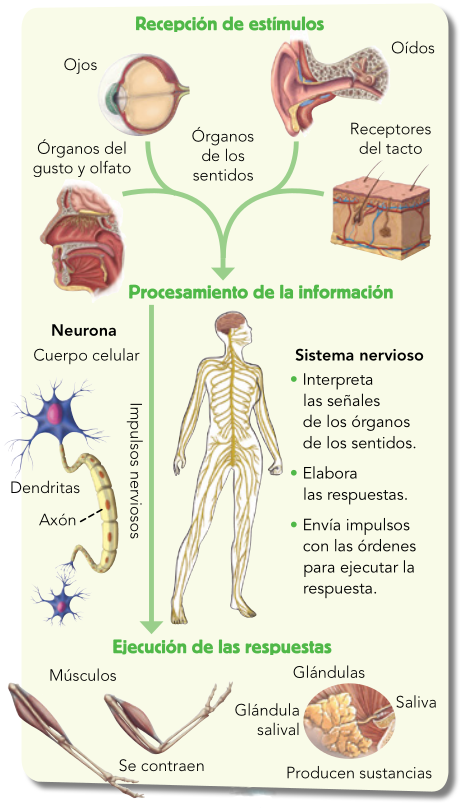
\includegraphics[width=0.4\linewidth]{Tema3/11_Relacion.png}
    \caption{La función de relación humana}
    \label{fig:relacion}
\end{figure}

\subsection{Los órganos receptores}

\subsubsection{Esquema básico de un órgano receptor}

Todos los órganos receptores (Figura \ref{fig:organos-receptores}) tienen un esquema básico común:

\begin{itemize}
    \item Una parte destinada a recibir el estímulo y muy especializada para captar un estímulo en particular.
    \item Unas células receptoras, que se encargan de transformar los estímulos en señales nerviosas.
    \item Unos nervios sensoriales, que envían esas señales al sistema nervioso para que las interprete.
\end{itemize}

\begin{figure}[!ht]
    \centering
    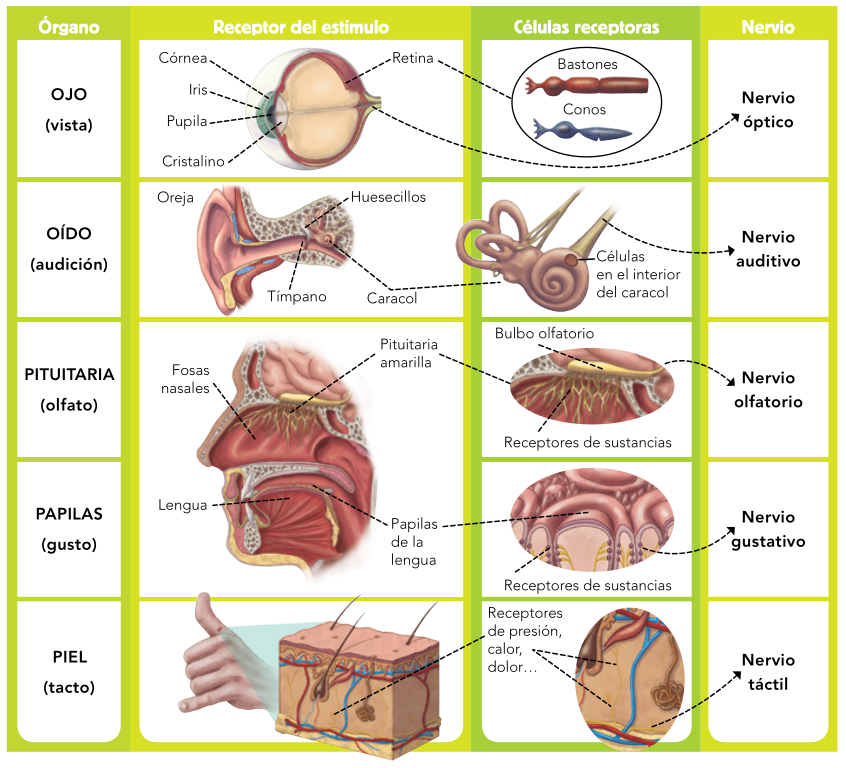
\includegraphics[width=0.6\linewidth]{Tema3/12_Organos_receptores.png}
    \caption{Esquema básico de los órganos receptores}
    \label{fig:organos-receptores}
\end{figure}

\subsection{El sistema nervioso}

El sistema nervioso (Figura \ref{fig:sistema-nervioso}) se organiza en dos partes: el sistema nervioso central y el sistema nervioso periférico.

\begin{figure}[!ht]
    \centering
    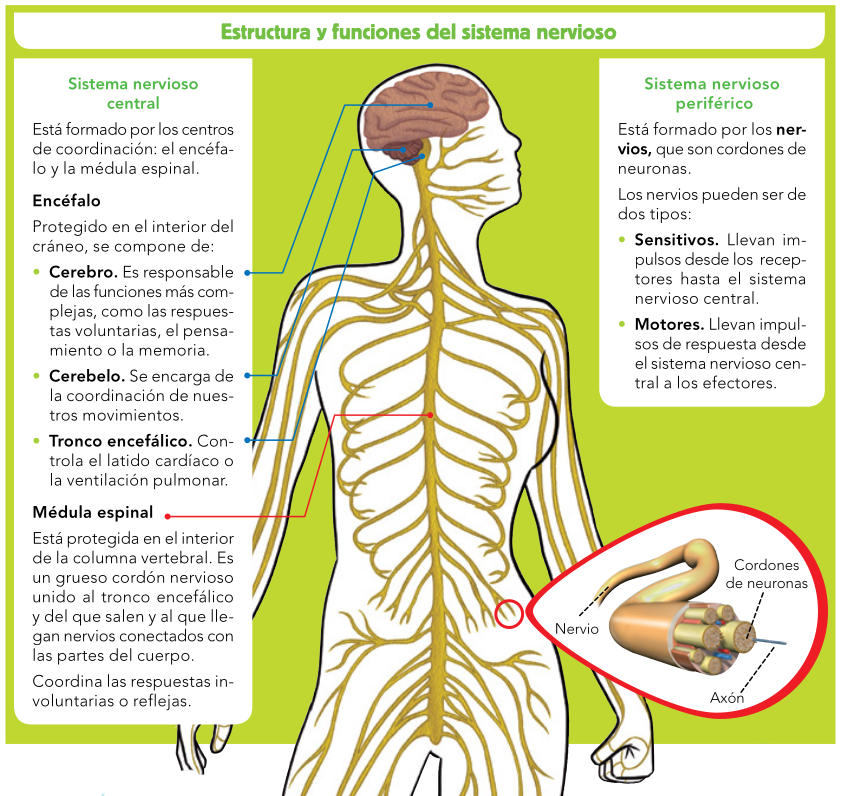
\includegraphics[width=0.6\linewidth]{Tema3/13_Estructura_funciones_sistema_nervioso.png}
    \caption{Estructura y funciones del sistema nervioso}
    \label{fig:sistema-nervioso}
\end{figure}

\subsubsection{Los órganos efectores}

Los órganos efectores son aquellos que realizan una acción cuando les llega una orden de respuesta a través del sistema nervioso. Los principales son los músculos y las glándulas.

\subsubsection{Los músculos}

Los músculos son órganos formados por células capaces de contraerse al recibir un impulso nervioso. De este modo, producen los movimientos del cuerpo.

\vspace{3mm}
Los seres humanos tenemos en nuestro cuerpo dos tipos de músculos:

\begin{itemize}
    \item \textbf{Músculos esqueléticos}. Como indica su nombre, funcionan en combinación con el esqueleto, están unidos a los huesos mediante tendones, y juntos constituyen el aparato locomotor. 
    \item \textbf{Músculos no esqueléticos}. Son músculos no relacionados con el esqueleto. Producen el movimiento de órganos como el corazón, el iris del ojo y el tubo digestivo.
\end{itemize}

\begin{figure}[!ht]
    \centering
    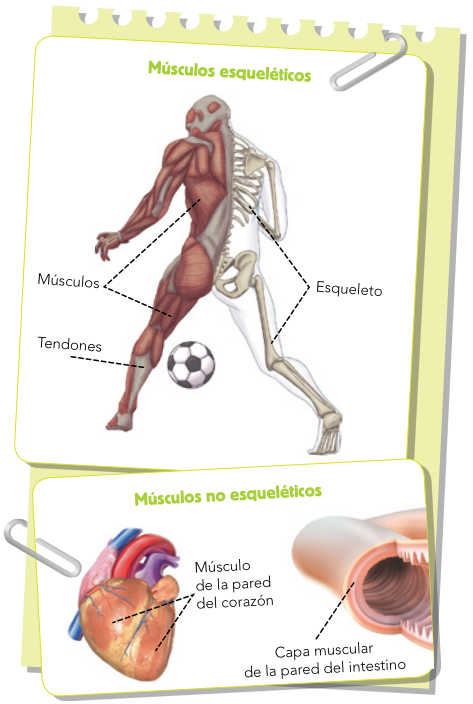
\includegraphics[width=0.5\linewidth]{Tema3/14_Musculos.png}
    \caption{Tipos de músculos}
    \label{fig:musculos}
\end{figure}

\subsubsection{Las glándulas}

Las glándulas son órganos que, cuando reciben una señal del sistema nervioso, producen determinadas sustancias como saliva, sudor, jugos digestivos, hormonas...

\subsection{Relación y salud}

El ambiente y ciertos malos hábitos pueden perjudicar a los órganos de los sentidos, al sistema nervioso o a los efectores, y alterar nuestra función de relación. Para prevenir algunos daños, además de ir a revisiones médicas periódicas, se pueden tomar ciertas medidas.

\subsubsection{El cuidado de los órganos de los sentidos}

Algunos hábitos saludables pueden prevenir enfermedades de los órganos de los sentidos:

\begin{itemize}
    \item \textbf{Cuidar la vista}. Conviene utilizar gafas de sol en la playa o la nieve, leer con suficiente luz, no pasar mucho tiempo mirando pantallas electrónicas, tomar alimentos con vitaminas, como frutas o verduras...
    \item \textbf{Cuidar los oídos}. Se debería evitar exponerse a ruidos fuertes o prolongados, introducir objetos en los oídos ni para secarlos, abusar de los auriculares...
    \item \textbf{Cuidar el olfato y el gusto}. Para ello, hay que mantener limpias tu boca y tus fosas nasales.
    \item \textbf{Cuidar el sentido del tacto}. Se consigue con una adecuada higiene de la piel y utilizando protección solar.
\end{itemize}

\subsubsection{El cuidado del sistema nervioso}

Debemos cuidar nuestro sistema nervioso tanto en el aspecto físico como en el emocional.

\vspace{3mm}
\textbf{El cuidado físico del sistema nervioso}

\begin{itemize}
    \item \textbf{Conviene protegerse de golpes} en la cabeza o la espalda, ya que el encéfalo o la columna podrían dañarse.
    \item \textbf{Hay que evitar siempre las bebidas alcohólicas, el tabaco y otras drogas}. Estas sustancias llegan al cerebro y pueden ocasionar daños en este órgano, especialmente en las personas jóvenes, como vosotras y vosotros, que estáis en pleno desarrollo.
\end{itemize}

\textbf{La salud emocional}

\vspace{3mm}
Para conseguir una buena salud emocional, es importante relacionarse con otras personas, \textbf{cuidar la autoestima, mostrar empatía,} adoptar una \textbf{actitud positiva}, intentar \textbf{superar las dificultades}...

\vspace{3mm}
\textbf{El cuidado de los efectores}

\vspace{3mm}
Para mantener en buen estado nuestro aparato locomotor, conviene seguir estos hábitos:

\begin{itemize}
    \item \textbf{Hacer ejercicio de forma regular} y adecuada para tu edad y tu fuerza. Asimismo, conviene realizar un calentamiento antes de empezar la actividad y unos estiramientos al finalizarla.
    \item \textbf{Mantener unas posturas que no dañen los músculos, la columna vertebral o las articulaciones} al caminar, al sentarse durante un tiempo, al cargar algo de peso...
    \item \textbf{Evitar las actividades con un exceso de peligro y utilizar protecciones adecuadas} al montar en bici, patinar, ir en coche...
\end{itemize}
\section{La función de reproducción humana}

La función de reproducción humana permite que las personas adultas puedan tener descendientes, es decir, hijas o hijos. La lleva a cabo el \textbf{aparato reproductor}.

\vspace{3mm}
\textbf{Nuestra reproducción es sexual}; es decir, que para tener lugar deben intervenir dos células reproductoras de distinto sexo: los \textbf{espermatozoides} y los \textbf{óvulos}. Estos dos tipos de células son producidas, respectivamente, por uno de los \textbf{dos tipos de aparato reproductor} que existen.

\vspace{3mm}
\textbf{La producción de espermatozoides} (Figura \ref{fig:reproductor-masculino})

\vspace{3mm}
El aparato reproductor que \textbf{se encarga de la producción de los espermatozoides}, es el que puedes ver a continuación:

\begin{figure}[!ht]
    \centering
    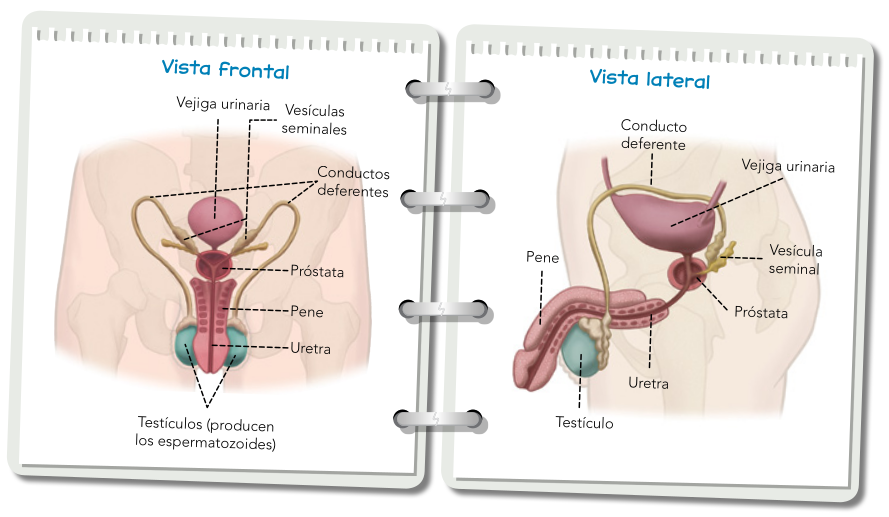
\includegraphics[width=0.7\linewidth]{Tema3/15_Aparato_reproductor_masculino.png}
    \caption{Aparato reproductor masculino}
    \label{fig:reproductor-masculino}
\end{figure}

\textbf{La producción de óvulos} (Figura \ref{fig:reproductor-femenino})

\vspace{3mm}
El aparato reproductor que \textbf{se encarga de la producción de los óvulos} es el que puedes ver en las imágenes de esta página. Además, está preparado para que en su interior tengan lugar la unión de las células reproductoras y el desarrollo del nuevo ser desde sus primeras etapas hasta su nacimiento.

\begin{figure}[!ht]
    \centering
    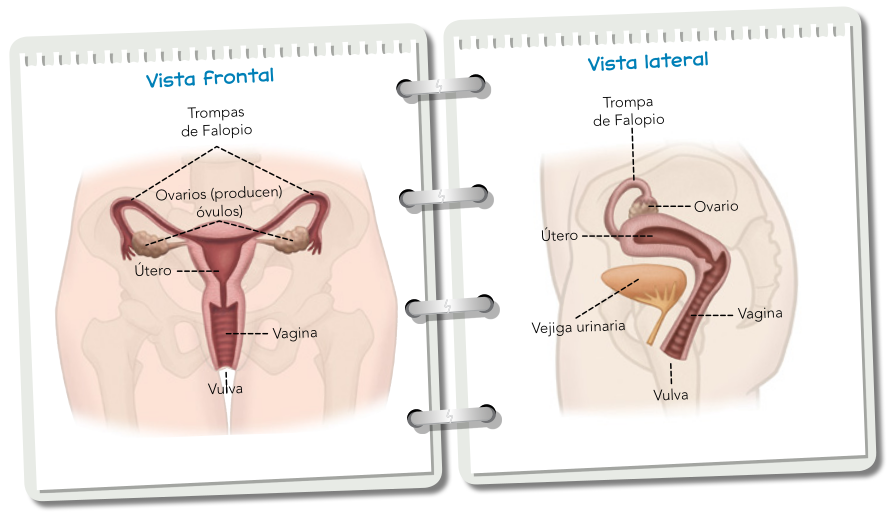
\includegraphics[width=0.7\linewidth]{Tema3/16_Aparato_reproductor_femenino.png}
    \caption{Aparato reproductor femenino}
    \label{fig:reproductor-femenino}
\end{figure}

\textbf{La pubertad}

\vspace{3mm}
Aunque nacemos con aparato reproductor, este no está completamente activo hasta cierta edad. Ese momento, que se produce entre los 10 y los 16 años, es el comienzo de la \textbf{pubertad}.

\begin{itemize}
    \item \textbf{Pubertad y producción de espermatozoides}. Cuando los testículos comienzan a producir espermatozoides, también segregan hormonas que causan la aparición del vello púbico y de la barba, el cambio del tono de voz, el desarrollo de una forma corporal más adulta...
    \item \textbf{Pubertad e inicio del ciclo menstrual}. Ocurre cuando los ovarios empiezan a liberar óvulos maduros, de uno en uno, más o menos cada 28 días. Esta liberación se llama \textbf{ovulación}. Es ahora cuando aparece la primera \textbf{regla o menstruación} y cuando se inicia la producción de hormonas que causan el desarrollo de vello púbico, de las mamas...
\end{itemize}

\subsection{El proceso de la reproducción}

El proceso de la reproducción en los seres humanos tiene lugar en tres fases: la \textbf{fecundación}, el \textbf{embarazo} y el \textbf{parto}.

\subsubsection{La fecundación}

La fecundación es la unión de las dos células reproductoras, el óvulo y el espermatozoide, para formar el cigoto, que es la célula que se desarrollará para formar el nuevo ser.

\vspace{3mm}
La fecundación suele tener lugar en el interior de las trompas de Falopio, mientras el óvulo está descendiendo desde el ovario que lo liberó. Sucede cuando un espermatozoide consigue entrar en el óvulo y los dos núcleos celulares se combinan.

\subsubsection{El embarazo}

El embarazo es el período que transcurre desde que se forma el cigoto hasta el nacimiento del bebé. Dura unos nueve meses y en él se producen numerosos cambios:

\vspace{3mm}
\textbf{El primer trimestre}

\vspace{3mm}
Tras la fecundación, el cigoto comienza a dividirse en varias células. Esto origina un \textbf{embrión}, que \textbf{se implanta} en el revestimiento de la pared del útero, llamado endometrio.

\vspace{3mm}
Poco después, alrededor del embrión se forma una membrana llena de líquido, el \textbf{saco amniótico}, donde queda protegido.

\vspace{3mm}
Al mismo tiempo se forma la \textbf{placenta}, que es un órgano que se conecta directamente a los vasos de la pared de útero. La placenta intercambia sustancias entre la sangre de la madre y el embrión a través del \textbf{cordón umbilical}.

\vspace{3mm}
\textbf{El segundo trimestre}

\vspace{3mm}
\textbf{El embrión pasa a llamarse feto}, crece y en él \textbf{comienzan a formarse casi todos los órganos}. Poco a poco adquiere un aspecto humano y comienza a realizar movimientos.

\vspace{3mm}
\textbf{El tercer trimestre}

\vspace{3mm}
\textbf{El feto prosigue su maduración y crecimiento}. A partir del séptimo mes, el desarrollo corporal es completo, aunque los pulmones o el aparato digestivo aún no están maduros. Hacia el noveno mes, el feto \textbf{se encaja}, es decir, se coloca con la cabeza hacia la salida del útero, preparándose para nacer.

\begin{figure}[!ht]
    \centering
    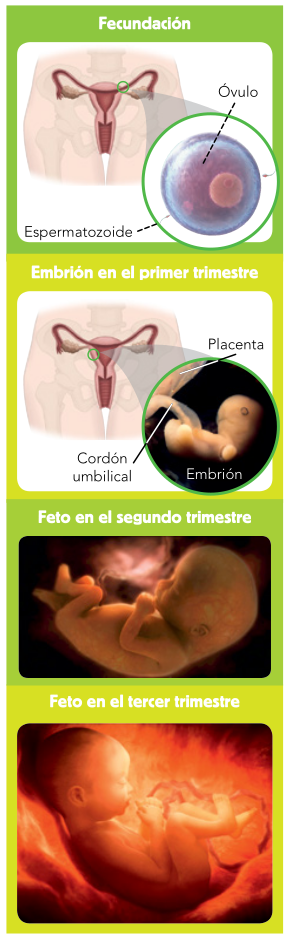
\includegraphics[width=0.3\linewidth]{Tema3/17_Proceso_reproduccion.png}
    \caption{El proceso de la reproducción}
    \label{fig:proceso-reproduccion}
\end{figure}

\subsubsection{El parto}

Cuando se acerca el momento del parto, \textbf{las paredes del útero comienzan a contraerse. El cuello del útero y la vagina se dilatan} para permitir la salida del feto.

\vspace{3mm}
Finalmente, \textbf{el saco amniótico se rompe} y el bebé y la placenta son expulsados al exterior. Los pulmones se activan y el bebé comienza a respirar.

\vspace{3mm}
Tras el nacimiento, el cordón umbilical debe ser cortado. El \textbf{ombligo} es la cicatriz que queda en el lugar del abdomen en el que el cordón estaba conectado al feto.

\vspace{3mm}
Como ocurre con otros mamíferos, \textbf{los bebés humanos están preparados para alimentarse de la leche que producen las mamas de la madre}. En esos primeros meses de vida continúa la maduración de su aparato digestivo y del sistema nervioso, que necesitan un tiempo para estar completamente operativos.

\subsection{Reproducción y salud}

\subsubsection{Pubertad y salud}

A vuestra edad, es posible que hayáis comenzado a experimentar los cambios de la pubertad, tanto físicos como mentales. Por eso conviene tener en cuenta algunos aspectos que pueden ayudar a mantener una salud adecuada.

\begin{itemize}
    \item \textbf{Cuidar la higiene personal} es importante a cualquier edad, pues contribuye a mantener un buen estado de salud. No obstante, los cambios de la pubertad pueden implicar que necesitéis prestar más atención a la higiene de vuestra piel o de las partes externas del aparato reproductor.
    \item \textbf{Respetar y exigir respeto}. Los cambios asociados a la pubertad no suceden de igual modo y al mismo tiempo en todas las personas. Puede que en vuestro grupo haya quien aún no haya empezado a cambiar y quien ya haya experimentado la mayor parte de los cambios. En estas circunstancias es muy importante el respeto mutuo.
    \item \textbf{Decidir de forma saludable por vuestra cuenta y no dejarse arrastrar por la presión del grupo}. Coincidiendo con la pubertad, seguramente experimentéis una serie de cambios en vuestra forma de ser. Os hacéis mayores y se empieza a definir vuestra personalidad. Las amistades cobran mucha importancia y el grupo ejerce mucha influencia. Es importante que sepáis decidir y actuar según lo que pensáis, teniendo en cuenta lo que es saludable, justo o respetuoso.
\end{itemize}


\chapter{Economía, sociedad y cultura en España y Europa}

\begin{figure}[!ht]
    \centering
    
\includegraphics[width=1\linewidth]{Tema4/00_Economia.jpg}
    \caption{Economía, sociedad y cultura en España y Europa}
    \label{fig:economia}
\end{figure}

\section{Las actividades económicas}

\subsection{La actividad económica}

Las personas, para satisfacer sus necesidades, como la alimentación, el vestido, los servicios (educación, sanidad, etc.), realizan una serie de tareas. A estas tareas las denominamos actividad económica. En esta se distinguen sus \textbf{componentes} (producción, distribución y consumo) y \textbf{quiénes la llevan a cabo} (empresas, familias...).

\subsubsection{Componentes de la actividad económica}

\textbf{Producción}

\vspace{3mm}
Es el conjunto de lo producido para satisfacer nuestras necesidades.

\vspace{3mm}
\textbf{Distribución}

\vspace{3mm}
Es el traslado de los productos producidos hasta las personas que los consumimos.

\vspace{3mm}
\textbf{Consumo}

\vspace{3mm}
Es el uso y disfrute de todo aquello proporcionado por la producción.

\subsubsection{¿Quiénes llevan a cabo la actividad económica?}

\textbf{Empresas}

\vspace{3mm}
Las \textbf{empresas} están formadas por una, varias o muchas personas. Se encargan de producir, distribuir y vender lo que necesitamos. Su fin es obtener beneficios. Se clasifican de distintas formas, como verás en la siguiente doble página.

\vspace{3mm}
\textbf{Personas, familias}

\vspace{3mm}
Las \textbf{personas o familias} son las consumidoras y los consumidores. \textbf{Compran} los bienes para satisfacer sus necesidades. Para ello \textbf{trabajan} en las empresas a cambio de recibir un salario con el que pagan los bienes y servicios que compran.

\subsubsection{¿Qué es necesario? Dinero y tipos de gastos}

Para el pago de productos y bienes que necesitamos, utilizamos el dinero, en forma de billetes o monedas.
En la Antigüedad, el trueque era el sistema utilizado para obtener lo que se necesitaba. Consistía en intercambiar los productos entre sí (gallinas por fruta, vacas por maíz, etc.). Con este sistema era muy difícil fijar el valor de cada producto. La aparición del \textbf{dinero} hizo que el comercio fuera más sencillo y permitió su expansión.

\vspace{3mm}
\textbf{Economía doméstica, nuestra economía}

\vspace{3mm}
Las personas o las familias, cada día, nos enfrentamos a distintos tipos de gastos (Figura \ref{fig:tipos-gastos}) para satisfacer nuestras necesidades, como son los fijos, los variables y los inesperados.

\begin{figure}[!ht]
    \centering
    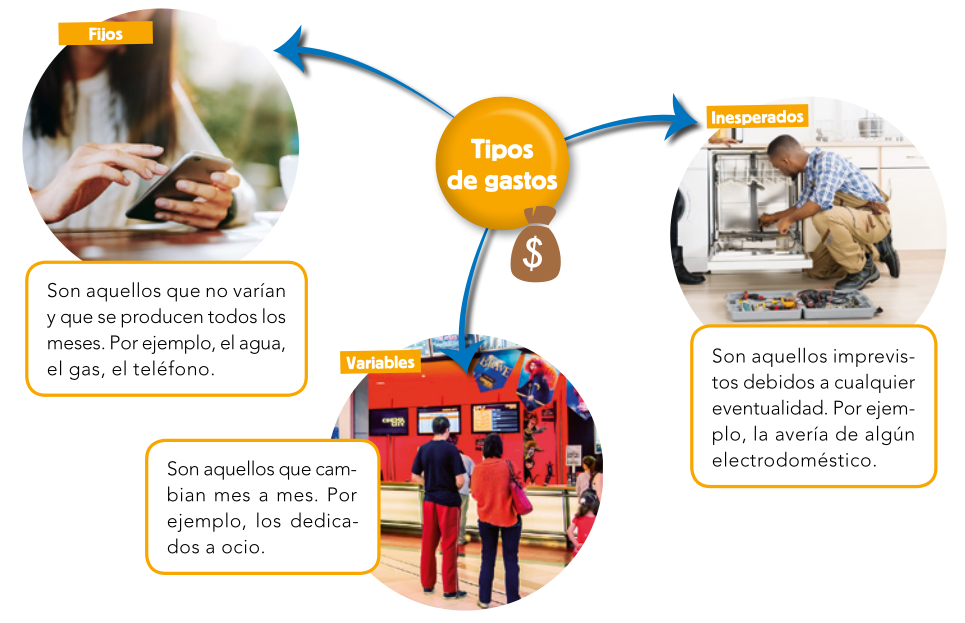
\includegraphics[width=1\linewidth]{Tema4/01_Tipos_gastos.png}
    \caption{Tipos de gastos}
    \label{fig:tipos-gastos}
\end{figure}

\vspace{3mm}
\textbf{Ahorro, publicidad y consumo responsable}

\vspace{3mm}
El \textbf{ahorro} es el dinero que no se destina al gasto y que se guarda para necesidades futuras. La clave del ahorro es la capacidad de juntar dinero de manera regular durante un periodo de tiempo. Antes de adquirir un producto, debemos valorar si realmente lo necesitamos y no dejarnos influenciar siempre por la \textbf{publicidad}, que intenta estimular su compra. Es decir, tenemos que realizar un \textbf{consumo responsable}.

\subsection{Las empresas y sus tipos}

Como ya has visto, las empresas se encargan de producir, distribuir y vender lo que necesitamos. Se pueden clasificar de muchas maneras: por su tipo de actividad (Figura \ref{fig:empresas-actividad}), por el lugar de donde procede el capital con el que se crean (Figura \ref{fig:empresas-capital}), por su tamaño (Figura \ref{fig:empresas-tamaño}), etc.

\begin{figure}[!ht]
    \centering
    \includegraphics[width=0.8\linewidth]{Tema4/02_Empresas_actividad.png}
    \caption{Empresas según su actividad}
    \label{fig:empresas-actividad}
\end{figure}

\begin{figure}[!ht]
    \centering
    \includegraphics[width=0.8\linewidth]{Tema4/01_Tipos_gastos.png}
    \caption{Empresas según de donde procede el capital}
    \label{fig:empresas-capital}
\end{figure}

\begin{figure}[!ht]
    \centering
    \includegraphics[width=0.8\linewidth]{Tema4/02_Empresas_actividad.png}
    \caption{Empresas según su tamaño}
    \label{fig:empresas-tamaño}
\end{figure}

\subsection{Sectores económicos. Sector primario}


\addcontentsline{toc}{chapter}{TRIMESTRE 3}

\part*{Trimestre 3}

\chapter{Materia y energía}

\include{Tema6_España}

\end{document}
